%
% file: localoperator.tex
% author: Victor Brena
% description: Briefly describes properties of the local operator.
%

\chapter{Appendix C: Issuer matched EUR/USD Dataset Analysis}
\label{appC}

%%%%%%%%%%%%%%%%%%%%%%%%%%%%%%%%%%%%%%%%%%%%%%%%%%%%%%%%%%%%
\section{C.1 Descriptive Statistics}
%%%%%%%%%%%%%%%%%%%%%%%%%%%%%%%%%%%%%%%%%%%%%%%%%%%%%%%%%%%%

%%%%%%%%%%%%%%%%%%%%%%%%%%%%%%%%%%%%%%%%%%%%%%%%%%%%%%%%%%%%
\subsection{C.1.1 Summary Statistics}
%%%%%%%%%%%%%%%%%%%%%%%%%%%%%%%%%%%%%%%%%%%%%%%%%%%%%%%%%%%%

%%%%%%%%%%%%%%%%%%%%%%%%%%%%%%%%%%%%%%%%%%%%%%%%%%%%%%%%%%%%
%\subsubsection{C.1.1.1 Green Bonds}
%%%%%%%%%%%%%%%%%%%%%%%%%%%%%%%%%%%%%%%%%%%%%%%%%%%%%%%%%%%%
% Table created by stargazer v.5.2.2 by Marek Hlavac, Harvard University. E-mail: hlavac at fas.harvard.edu
% Date and time: Fri, Nov 11, 2022 - 17:55:33
\begin{table}[!h] \centering 
  \footnotesize
  \caption{Data Matched USDEUR Green Bond Summary Statistics} 
  \label{desc3} 
\begin{tabular}{@{\extracolsep{5pt}}lccccccc} 
\\[-1.8ex]\hline 
\hline \\[-1.8ex] 
Statistic & \multicolumn{1}{c}{N} & \multicolumn{1}{c}{Mean} & \multicolumn{1}{c}{St. Dev.} & \multicolumn{1}{c}{Min} & \multicolumn{1}{c}{Pctl(25)} & \multicolumn{1}{c}{Pctl(75)} & \multicolumn{1}{c}{Max} \\ 
\hline \\[-1.8ex] 
Time to Maturity (Days) & 663 & 2,997.576 & 1,968.983 & 367 & 1,833 & 3,660 & 18,269 \\ 
Issue Amount & 663 & 1,396.167 & 2,145.963 & 500.000 & 571.474 & 1,242.435 & 33,563.640 \\ 
Coupon Rate & 663 & 1.263 & 1.211 & 0.000 & 0.375 & 1.812 & 9.500 \\ 
Guarantor & 663 & 0.140 & 0.348 & 0 & 0 & 0 & 1 \\ 
Offer Yield to Maturity & 663 & 1.306 & 1.224 & $-$0.403 & 0.440 & 1.893 & 9.500 \\ 
Green Flag & 663 & 1.000 & 0.000 & 1 & 1 & 1 & 1 \\ 
2008 & 663 & 0.000 & 0.000 & 0 & 0 & 0 & 0 \\ 
2009 & 663 & 0.000 & 0.000 & 0 & 0 & 0 & 0 \\ 
2010 & 663 & 0.000 & 0.000 & 0 & 0 & 0 & 0 \\ 
2011 & 663 & 0.000 & 0.000 & 0 & 0 & 0 & 0 \\ 
2012 & 663 & 0.002 & 0.039 & 0 & 0 & 0 & 1 \\ 
2013 & 663 & 0.012 & 0.109 & 0 & 0 & 0 & 1 \\ 
2014 & 663 & 0.012 & 0.109 & 0 & 0 & 0 & 1 \\ 
2015 & 663 & 0.038 & 0.191 & 0 & 0 & 0 & 1 \\ 
2016 & 663 & 0.048 & 0.214 & 0 & 0 & 0 & 1 \\ 
2017 & 663 & 0.078 & 0.269 & 0 & 0 & 0 & 1 \\ 
2018 & 663 & 0.086 & 0.281 & 0 & 0 & 0 & 1 \\ 
2019 & 663 & 0.130 & 0.336 & 0 & 0 & 0 & 1 \\ 
2020 & 663 & 0.164 & 0.371 & 0 & 0 & 0 & 1 \\ 
2021 & 663 & 0.237 & 0.425 & 0 & 0 & 0 & 1 \\ 
2022 & 663 & 0.193 & 0.395 & 0 & 0 & 0 & 1 \\ 
AAA & 663 & 0.312 & 0.464 & 0 & 0 & 1 & 1 \\ 
AA & 663 & 0.214 & 0.411 & 0 & 0 & 0 & 1 \\ 
A & 663 & 0.228 & 0.420 & 0 & 0 & 0 & 1 \\ 
BBB & 663 & 0.229 & 0.421 & 0 & 0 & 0 & 1 \\ 
BB & 663 & 0.014 & 0.116 & 0 & 0 & 0 & 1 \\ 
B & 663 & 0.003 & 0.055 & 0 & 0 & 0 & 1 \\ 
EUR & 663 & 0.688 & 0.464 & 0 & 0 & 1 & 1 \\ 
USD & 663 & 0.312 & 0.464 & 0 & 0 & 1 & 1 \\ 
Annual Coupon & 663 & 0.716 & 0.451 & 0 & 0 & 1 & 1 \\ 
Semi Annual Coupon & 663 & 0.282 & 0.450 & 0 & 0 & 1 & 1 \\ 
Quarterly & 663 & 0.000 & 0.000 & 0 & 0 & 0 & 0 \\ 
Maturity & 663 & 0.002 & 0.039 & 0 & 0 & 0 & 1 \\
\hline \\[-1.8ex] 
\end{tabular} 
\end{table} 

\newpage

\begin{table}[!htbp] \centering 
  \footnotesize
  \caption{Data Matched USDEUR Green Bond Summary Statistics cont.} 
  \label{} 
\begin{tabular}{@{\extracolsep{5pt}}lccccccc} 
\\[-1.8ex]\hline 
\hline \\[-1.8ex] 
Statistic & \multicolumn{1}{c}{N} & \multicolumn{1}{c}{Mean} & \multicolumn{1}{c}{St. Dev.} & \multicolumn{1}{c}{Min} & \multicolumn{1}{c}{Pctl(25)} & \multicolumn{1}{c}{Pctl(75)} & \multicolumn{1}{c}{Max} \\ 
\hline \\[-1.8ex] 
Basic Materials & 663 & 0.015 & 0.122 & 0 & 0 & 0 & 1 \\ 
Consumer Cyclicals & 663 & 0.006 & 0.077 & 0 & 0 & 0 & 1 \\ 
Consumer Non-Cyclicals & 663 & 0.008 & 0.087 & 0 & 0 & 0 & 1 \\
Energy & 663 & 0.003 & 0.055 & 0 & 0 & 0 & 1 \\ 
Financials & 663 & 0.596 & 0.491 & 0 & 0 & 1 & 1 \\ 
Government Activity & 663 & 0.195 & 0.396 & 0 & 0 & 0 & 1 \\ 
Healthcare & 663 & 0.003 & 0.055 & 0 & 0 & 0 & 1 \\ 
Industrials & 663 & 0.033 & 0.179 & 0 & 0 & 0 & 1 \\ 
Institutions, Associations \& Organizations & 663 & 0.066 & 0.249 & 0 & 0 & 0 & 1 \\ 
Real Estate & 663 & 0.020 & 0.139 & 0 & 0 & 0 & 1 \\ 
Technology & 663 & 0.006 & 0.077 & 0 & 0 & 0 & 1 \\ 
Utilities & 663 & 0.050 & 0.218 & 0 & 0 & 0 & 1 \\ 
Senior Secured Mortgage & 663 & 0.069 & 0.254 & 0 & 0 & 0 & 1 \\ 
Senior Secured & 663 & 0.026 & 0.158 & 0 & 0 & 0 & 1 \\ 
Senior Unsecured & 663 & 0.732 & 0.444 & 0 & 0 & 1 & 1 \\ 
Senior Non-Preferred & 663 & 0.060 & 0.238 & 0 & 0 & 0 & 1 \\ 
Senior Preferred & 663 & 0.077 & 0.267 & 0 & 0 & 0 & 1 \\ 
Senior Subordinated Unsecured & 663 & 0.002 & 0.039 & 0 & 0 & 0 & 1 \\ 
Subordinated Unsecured & 663 & 0.008 & 0.087 & 0 & 0 & 0 & 1 \\ 
Unsecured & 663 & 0.026 & 0.158 & 0 & 0 & 0 & 1 \\ 
Public Sector & 663 & 0.460 & 0.499 & 0 & 0 & 1 & 1 \\ 
Corporate Sector & 663 & 0.540 & 0.499 & 0 & 0 & 1 & 1 \\ 
\hline \\[-1.8ex] 
\end{tabular} 
\end{table} 

%%%%%%%%%%%%%%%%%%%%%%%%%%%%%%%%%%%%%%%%%%%%%%%%%%%%%%%%%%%%
%\subsubsection{C.1.1.2 Brown Bonds}
%%%%%%%%%%%%%%%%%%%%%%%%%%%%%%%%%%%%%%%%%%%%%%%%%%%%%%%%%%%%

% Table created by stargazer v.5.2.2 by Marek Hlavac, Harvard University. E-mail: hlavac at fas.harvard.edu
% Date and time: Fri, Nov 11, 2022 - 17:55:33
\begin{table}[!htbp] \centering 
  \footnotesize
  \caption{Data Matched USDEUR Brown Bond Summary Statistics} 
  \label{} 
\begin{tabular}{@{\extracolsep{5pt}}lccccccc} 
\\[-1.8ex]\hline 
\hline \\[-1.8ex] 
Statistic & \multicolumn{1}{c}{N} & \multicolumn{1}{c}{Mean} & \multicolumn{1}{c}{St. Dev.} & \multicolumn{1}{c}{Min} & \multicolumn{1}{c}{Pctl(25)} & \multicolumn{1}{c}{Pctl(75)} & \multicolumn{1}{c}{Max} \\ 
\hline \\[-1.8ex] 
Time to Maturity (Days) & 4,349 & 2,632.082 & 2,248.019 & 373 & 1,759 & 3,613 & 36,532 \\ 
Issue Amount & 4,349 & 1,631.361 & 1,491.449 & 500 & 838.7 & 1,775.0 & 30,089 \\ 
Coupon Rate & 4,349 & 2.117 & 1.525 & 0.010 & 0.875 & 3.000 & 9.000 \\ 
Guarantor & 4,349 & 0.187 & 0.390 & 0 & 0 & 0 & 1 \\ 
Offer Yield to Maturity & 4,349 & 2.152 & 1.530 & 0.004 & 0.942 & 3.060 & 9.000 \\ 
Green Flag & 4,349 & 0.000 & 0.000 & 0 & 0 & 0 & 0 \\ 
2008 & 4,349 & 0.046 & 0.209 & 0 & 0 & 0 & 1 \\ 
2009 & 4,349 & 0.054 & 0.226 & 0 & 0 & 0 & 1 \\ 
2010 & 4,349 & 0.070 & 0.255 & 0 & 0 & 0 & 1 \\ 
2011 & 4,349 & 0.074 & 0.262 & 0 & 0 & 0 & 1 \\ 
2012 & 4,349 & 0.088 & 0.283 & 0 & 0 & 0 & 1 \\ 
2013 & 4,349 & 0.079 & 0.269 & 0 & 0 & 0 & 1 \\ 
\hline \\[-1.8ex] 
\end{tabular} 
\end{table} 


\begin{table}[!htbp] \centering 
  \footnotesize
  \caption{Data Matched USDEUR Brown Bond Summary Statistics cont.} 
  \label{} 
\begin{tabular}{@{\extracolsep{5pt}}lccccccc} 
\\[-1.8ex]\hline 
\hline \\[-1.8ex] 
Statistic & \multicolumn{1}{c}{N} & \multicolumn{1}{c}{Mean} & \multicolumn{1}{c}{St. Dev.} & \multicolumn{1}{c}{Min} & \multicolumn{1}{c}{Pctl(25)} & \multicolumn{1}{c}{Pctl(75)} & \multicolumn{1}{c}{Max} \\ 
\hline \\[-1.8ex] 
2014 & 4,349 & 0.077 & 0.267 & 0 & 0 & 0 & 1 \\ 
2015 & 4,349 & 0.082 & 0.275 & 0 & 0 & 0 & 1 \\ 
2016 & 4,349 & 0.084 & 0.277 & 0 & 0 & 0 & 1 \\ 
2017 & 4,349 & 0.072 & 0.259 & 0 & 0 & 0 & 1 \\ 
2018 & 4,349 & 0.068 & 0.252 & 0 & 0 & 0 & 1 \\ 
2019 & 4,349 & 0.073 & 0.260 & 0 & 0 & 0 & 1 \\ 
2020 & 4,349 & 0.048 & 0.214 & 0 & 0 & 0 & 1 \\ 
2021 & 4,349 & 0.037 & 0.188 & 0 & 0 & 0 & 1 \\ 
2022 & 4,349 & 0.047 & 0.212 & 0 & 0 & 0 & 1 \\ 
AAA & 4,349 & 0.458 & 0.498 & 0 & 0 & 1 & 1 \\ 
AA & 4,349 & 0.254 & 0.435 & 0 & 0 & 1 & 1 \\ 
A & 4,349 & 0.139 & 0.346 & 0 & 0 & 0 & 1 \\ 
BBB & 4,349 & 0.133 & 0.340 & 0 & 0 & 0 & 1 \\ 
BB & 4,349 & 0.013 & 0.114 & 0 & 0 & 0 & 1 \\ 
B & 4,349 & 0.002 & 0.048 & 0 & 0 & 0 & 1 \\ 
EUR & 4,349 & 0.599 & 0.490 & 0 & 0 & 1 & 1 \\ 
USD & 4,349 & 0.401 & 0.490 & 0 & 0 & 1 & 1 \\ 
Annual Coupon & 4,349 & 0.652 & 0.477 & 0 & 0 & 1 & 1 \\ 
Semi Annual Coupon & 4,349 & 0.346 & 0.476 & 0 & 0 & 1 & 1 \\ 
Quarterly & 4,349 & 0.002 & 0.040 & 0 & 0 & 0 & 1 \\ 
Maturity & 4,349 & 0.001 & 0.026 & 0 & 0 & 0 & 1 \\ 
Basic Materials & 4,349 & 0.006 & 0.074 & 0 & 0 & 0 & 1 \\ 
Consumer Cyclicals & 4,349 & 0.005 & 0.073 & 0 & 0 & 0 & 1 \\ 
Consumer Non-Cyclicals & 4,349 & 0.002 & 0.045 & 0 & 0 & 0 & 1 \\ 
Energy & 4,349 & 0.006 & 0.076 & 0 & 0 & 0 & 1 \\ 
Financials & 4,349 & 0.705 & 0.456 & 0 & 0 & 1 & 1 \\ 
Government Activity & 4,349 & 0.211 & 0.408 & 0 & 0 & 0 & 1 \\ 
Healthcare & 4,349 & 0.001 & 0.026 & 0 & 0 & 0 & 1 \\ 
Industrials & 4,349 & 0.008 & 0.087 & 0 & 0 & 0 & 1 \\ 
Institutions, Associations \& Organizations & 4,349 & 0.036 & 0.187 & 0 & 0 & 0 & 1 \\ 
Real Estate & 4,349 & 0.001 & 0.030 & 0 & 0 & 0 & 1 \\ 
Technology & 4,349 & 0.007 & 0.083 & 0 & 0 & 0 & 1 \\ 
Utilities & 4,349 & 0.014 & 0.116 & 0 & 0 & 0 & 1 \\ 
Senior Secured Mortgage & 4,349 & 0.100 & 0.300 & 0 & 0 & 0 & 1 \\ 
Senior Secured & 4,349 & 0.057 & 0.231 & 0 & 0 & 0 & 1 \\ 
Senior Unsecured & 4,349 & 0.647 & 0.478 & 0 & 0 & 1 & 1 \\ 
Senior Non-Preferred & 4,349 & 0.029 & 0.168 & 0 & 0 & 0 & 1 \\ 
Senior Preferred & 4,349 & 0.051 & 0.220 & 0 & 0 & 0 & 1 \\ 
Senior Subordinated Unsecured & 4,349 & 0.003 & 0.052 & 0 & 0 & 0 & 1 \\ 
Subordinated Unsecured & 4,349 & 0.023 & 0.148 & 0 & 0 & 0 & 1 \\ 
Unsecured & 4,349 & 0.073 & 0.261 & 0 & 0 & 0 & 1 \\ 
Public Sector & 4,349 & 0.487 & 0.500 & 0 & 0 & 1 & 1 \\ 
Corporate Sector & 4,349 & 0.513 & 0.500 & 0 & 0 & 1 & 1 \\ 
\hline \\[-1.8ex] 
\end{tabular} 
\end{table} 

\newpage

%%%%%%%%%%%%%%%%%%%%%%%%%%%%%%%%%%%%%%%%%%%%%%%%%%%%%%%%%%%%
\subsection{C.1.2 Raincloud Plots}
%%%%%%%%%%%%%%%%%%%%%%%%%%%%%%%%%%%%%%%%%%%%%%%%%%%%%%%%%%%%

\begin{figure}[h!]
    \centering
    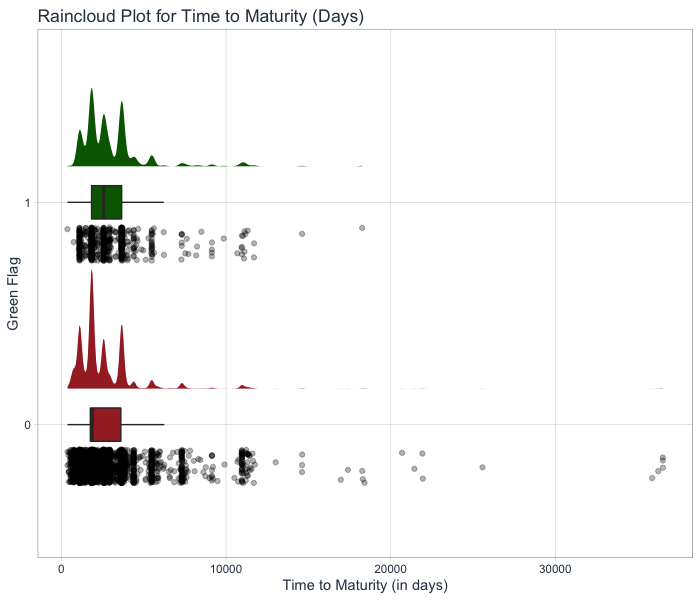
\includegraphics[scale=0.45]{chinchilab-template/chapters/appendices/ANALYSIS/raincloud3_ttm.png}
    \caption{Raincloud Plot for Time to Maturity (Days)}
    \label{fig:my_label}
\end{figure}

\begin{figure}[h!]
    \centering
    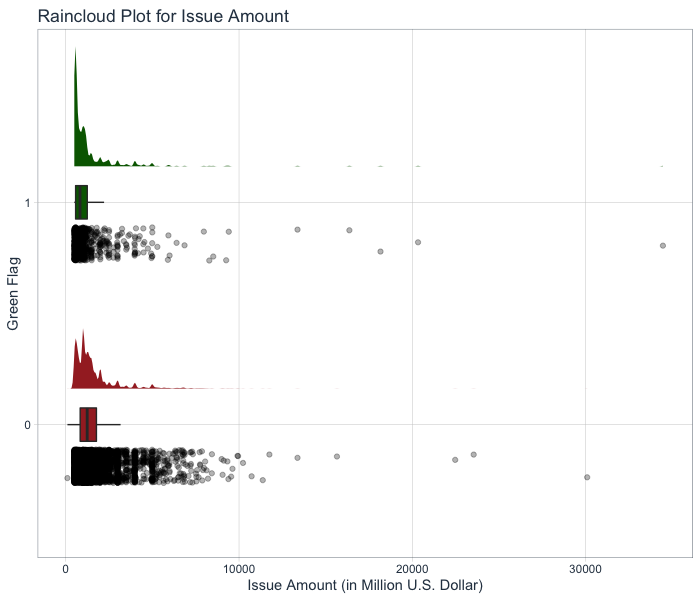
\includegraphics[scale=0.45]{chinchilab-template/chapters/appendices/ANALYSIS/raincloud3_size.png}
    \caption{Raincloud for Issue Amount}
    \label{fig:my_label}
\end{figure}

\begin{figure}[h!]
    \centering
    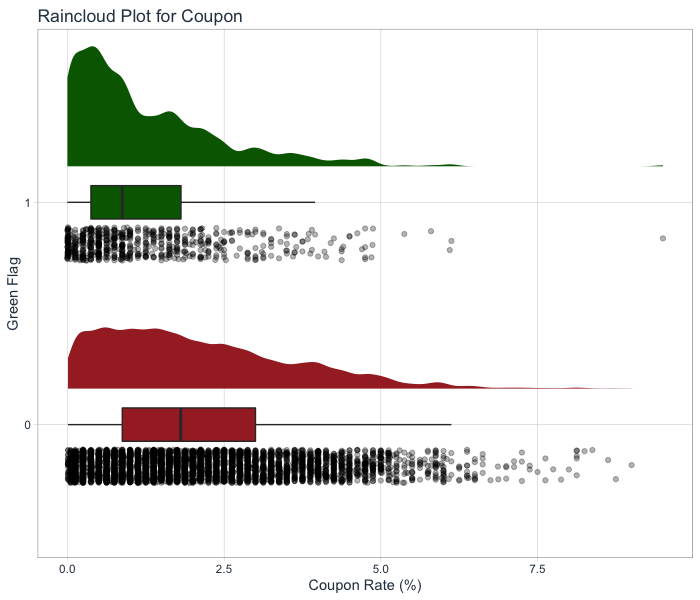
\includegraphics[scale=0.47]{chinchilab-template/chapters/appendices/ANALYSIS/raincloud3_coupon.png}
    \caption{Raincloud for Coupon Rate}
    \label{fig:my_label}
\end{figure}

\begin{figure}[h!]
    \centering
    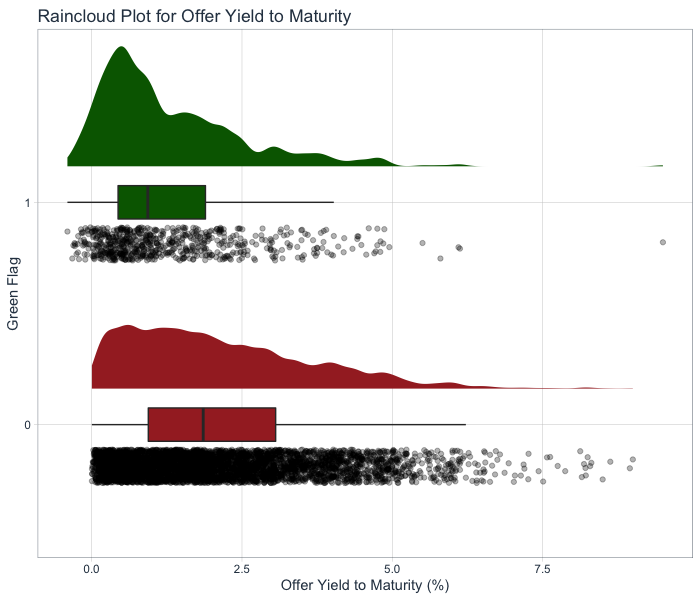
\includegraphics[scale=0.47]{chinchilab-template/chapters/appendices/ANALYSIS/raincloud3_oytm.png}
    \caption{Raincloud for Issuance Yield}
    \label{fig:my_label}
\end{figure}

\newpage

%%%%%%%%%%%%%%%%%%%%%%%%%%%%%%%%%%%%%%%%%%%%%%%%%%%%%%%%%%%%
\subsection{C.1.3 Correlation}
%%%%%%%%%%%%%%%%%%%%%%%%%%%%%%%%%%%%%%%%%%%%%%%%%%%%%%%%%%%%

\begin{figure}[h!]
    \centering
    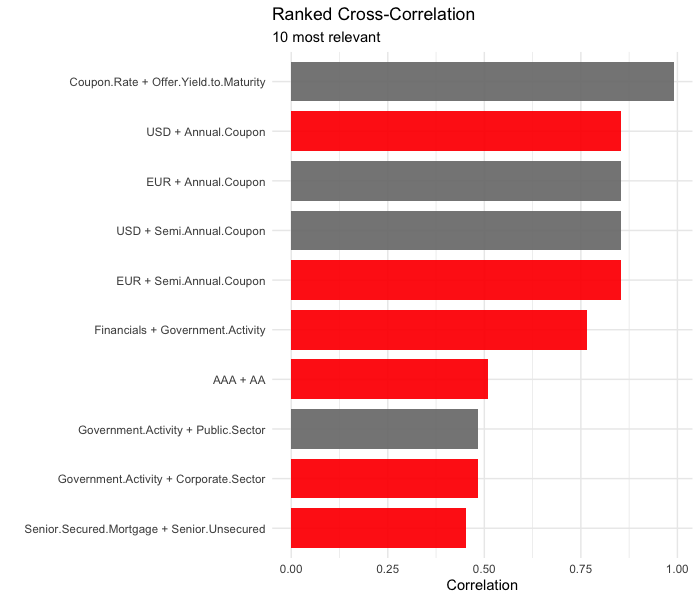
\includegraphics[scale=0.45]{chinchilab-template/chapters/appendices/ANALYSIS/correlation3.png}
    \caption{Ranked Cross-Correlation of 10 Most Relevant Pairs}
    \caption*{Note: Blue = Positive Correlation, Red = Negative Correlation.}
    \label{fig:my_label}
\end{figure}

%%%%%%%%%%%%%%%%%%%%%%%%%%%%%%%%%%%%%%%%%%%%%%%%%%%%%%%%%%%%
\subsection{C.1.4 Propensity Tables}
%%%%%%%%%%%%%%%%%%%%%%%%%%%%%%%%%%%%%%%%%%%%%%%%%%%%%%%%%%%%

\begin{table}[H]{
    \begin{subtable}{.5\textwidth}
    \footnotesize
    \centering
        {\begin{tabular}{lll}
        \\[-1.8ex]\hline 
        \hline \\[-1.8ex] 
        \textbf{Issue Year} & \textbf{Green (\%)} & \textbf{Brown (\%)} \\
        \hline \\[-1.8ex]
        2008 & \cellcolor[HTML]{FFFFFF}0.0 & \cellcolor[HTML]{D6E3D1}4.6 \\
        \cellcolor[HTML]{FAFAFA}2009 & \cellcolor[HTML]{FFFFFF}0.0 & \cellcolor[HTML]{B1CAA9}5.4 \\
        2010 & \cellcolor[HTML]{FFFFFF}0.0 & \cellcolor[HTML]{6A995C}7.0 \\
        \cellcolor[HTML]{FAFAFA}2011 & \cellcolor[HTML]{FFFFFF}0.0 & \cellcolor[HTML]{588D4A}{\color[HTML]{FFFFFF} 7.4} \\
        2012 & \cellcolor[HTML]{FDFEFD}0.2 & \cellcolor[HTML]{006400}{\color[HTML]{FFFFFF} 8.8} \\
        \cellcolor[HTML]{FAFAFA}2013 & \cellcolor[HTML]{F3F7F2}1.2 & \cellcolor[HTML]{407E33}{\color[HTML]{FFFFFF} 7.9} \\
        2014 & \cellcolor[HTML]{F3F7F2}1.2 & \cellcolor[HTML]{4A843C}{\color[HTML]{FFFFFF} 7.7} \\
        \cellcolor[HTML]{FAFAFA}2015 & \cellcolor[HTML]{D9E5D5}3.8 & \cellcolor[HTML]{307624}{\color[HTML]{FFFFFF} 8.2} \\
        2016 & \cellcolor[HTML]{D0DFCA}4.8 & \cellcolor[HTML]{25701A}{\color[HTML]{FFFFFF} 8.4} \\
        \cellcolor[HTML]{FAFAFA}2017 & \cellcolor[HTML]{B2CBAA}7.8 & \cellcolor[HTML]{619353}{\color[HTML]{FFFFFF} 7.2} \\
        2018 & \cellcolor[HTML]{ABC5A1}8.6 & \cellcolor[HTML]{739F66}6.8 \\
        \cellcolor[HTML]{FAFAFA}2019 & \cellcolor[HTML]{80A874}13.0 & \cellcolor[HTML]{5C904E}{\color[HTML]{FFFFFF} 7.3} \\
        2020 & \cellcolor[HTML]{609252}{\color[HTML]{FFFFFF} 16.4} & \cellcolor[HTML]{CDDDC6}4.8 \\
        \cellcolor[HTML]{FAFAFA}2021 & \cellcolor[HTML]{006400}{\color[HTML]{FFFFFF} 23.7} & \cellcolor[HTML]{FFFFFF}3.7 \\
        2022 & \cellcolor[HTML]{428035}{\color[HTML]{FFFFFF} 19.3} & \cellcolor[HTML]{D1E0CB}4.7 \\
        \hline \\[-1.8ex]
        \end{tabular}}
    \subcaption{Issue Year}
    \label{propyear}
    \end{subtable}
    \begin{subtable}{0.3\linewidth}
    \footnotesize
    \centering
        {\begin{tabular}{lll}
        \\[-1.8ex]\hline 
        \hline \\[-1.8ex] 
        \textbf{Rating} & \textbf{Green (\%)} & \textbf{Brown (\%)} \\
        \hline \\[-1.8ex]
        AAA & \cellcolor[HTML]{006400}{\color[HTML]{FFFFFF} 31.2} & \cellcolor[HTML]{006400}{\color[HTML]{FFFFFF} 45.8} \\
        \cellcolor[HTML]{FAFAFA}AA & \cellcolor[HTML]{619353}{\color[HTML]{FFFFFF} 21.4} & \cellcolor[HTML]{7FA872}25.4 \\
        A & \cellcolor[HTML]{568D49}{\color[HTML]{FFFFFF} 22.8} & \cellcolor[HTML]{B8CFB0}13.9 \\
        \cellcolor[HTML]{FAFAFA}BBB & \cellcolor[HTML]{568C48}{\color[HTML]{FFFFFF} 22.9} & \cellcolor[HTML]{BBD1B3}13.3 \\
        BB & \cellcolor[HTML]{F4F8F3}1.4 & \cellcolor[HTML]{F8FAF7}1.3 \\
        \cellcolor[HTML]{FAFAFA}B & \cellcolor[HTML]{FDFDFC}0.3 & \cellcolor[HTML]{FEFEFE}0.2 \\
        CCC & \cellcolor[HTML]{FFFFFF}0.0 & \cellcolor[HTML]{FFFFFF}0.0 \\
        \hline \\[-1.8ex]
        \end{tabular}}
    \subcaption{Rating}
    \label{proprating}
    \end{subtable}
\caption{Propensity Tables}}
\end{table}

\begin{table}[h!]
\centering
\caption{Propensity Table for Coupon Frequency}
\footnotesize
\begin{tabular}{lll}
\\[-1.8ex]\hline 
\hline \\[-1.8ex] 
\cellcolor[HTML]{FFFFFF}{\color[HTML]{333333} \textbf{Coupon Frequency}} & {\color[HTML]{333333} \textbf{Green (\%)}} & {\color[HTML]{333333} \textbf{Brown (\%)}} \\
\hline \\[-1.8ex] 
Annual Coupon & \cellcolor[HTML]{006400}{\color[HTML]{FFFFFF} 71.6} & \cellcolor[HTML]{006400}{\color[HTML]{FFFFFF} 65.2} \\
\cellcolor[HTML]{FAFAFA}Semi Annual Coupon & \cellcolor[HTML]{A4C099}28.2 & \cellcolor[HTML]{85AB78}34.6 \\
Quarterly & \cellcolor[HTML]{FFFFFF}0.0 & 0.2 \\
\cellcolor[HTML]{FAFAFA}Maturity & \cellcolor[HTML]{FEFFFE}0.2 & 0.1 \\
\hline \\[-1.8ex] 
\end{tabular}
\end{table}

\begin{table}[h!] \centering
\caption{Propensity Table for Industry}
\footnotesize
\begin{tabular}{lll}
\\[-1.8ex]\hline 
\hline \\[-1.8ex] 
\cellcolor[HTML]{FFFFFF}{\color[HTML]{333333} \textbf{TRBC Industry}} & \cellcolor[HTML]{FFFFFF}{\color[HTML]{333333} \textbf{Green (\%)}} & \cellcolor[HTML]{FFFFFF}{\color[HTML]{333333} \textbf{Brown (\%)}} \\
\hline \\[-1.8ex] 
\rowcolor[HTML]{FFFFFF} 
{\color[HTML]{333333} Academic \& Educational Services} & {\color[HTML]{333333} 0.0} & {\color[HTML]{333333} 0.0} \\
\cellcolor[HTML]{FAFAFA}{\color[HTML]{333333} Basic Materials} & \cellcolor[HTML]{F9FBF8}{\color[HTML]{333333} 1.5} & \cellcolor[HTML]{FDFEFD}{\color[HTML]{333333} 0.6} \\
\cellcolor[HTML]{FFFFFF}{\color[HTML]{333333} Consumer Cyclicals} & \cellcolor[HTML]{FDFDFC}{\color[HTML]{333333} 0.6} & \cellcolor[HTML]{FDFEFD}{\color[HTML]{333333} 0.5} \\
\cellcolor[HTML]{FAFAFA}{\color[HTML]{333333} Consumer Non-Cyclicals} & \cellcolor[HTML]{FCFDFB}{\color[HTML]{333333} 0.8} & \cellcolor[HTML]{FEFFFE}{\color[HTML]{333333} 0.2} \\
\cellcolor[HTML]{FFFFFF}{\color[HTML]{333333} Energy} & \cellcolor[HTML]{FEFEFE}{\color[HTML]{333333} 0.3} & \cellcolor[HTML]{FDFEFD}{\color[HTML]{333333} 0.6} \\
\rowcolor[HTML]{006400} 
\cellcolor[HTML]{FAFAFA}{\color[HTML]{333333} Financials} & {\color[HTML]{FFFFFF} 59.6} & {\color[HTML]{FFFFFF} 70.5} \\
\cellcolor[HTML]{FFFFFF}{\color[HTML]{333333} Government Activity} & \cellcolor[HTML]{B3CBAA}{\color[HTML]{333333} 19.5} & \cellcolor[HTML]{B9CFB1}{\color[HTML]{333333} 21.1} \\
\cellcolor[HTML]{FAFAFA}{\color[HTML]{333333} Healthcare} & \cellcolor[HTML]{FEFEFE}{\color[HTML]{333333} 0.3} & \cellcolor[HTML]{FFFFFF}{\color[HTML]{333333} 0.1} \\
\cellcolor[HTML]{FFFFFF}{\color[HTML]{333333} Industrials} & \cellcolor[HTML]{F2F6F0}{\color[HTML]{333333} 3.3} & \cellcolor[HTML]{FCFDFC}{\color[HTML]{333333} 0.8} \\
\cellcolor[HTML]{FAFAFA}{\color[HTML]{333333} Institutions, Associations \& Organizations} & \cellcolor[HTML]{E5EDE2}{\color[HTML]{333333} 6.6} & \cellcolor[HTML]{F2F6F1}{\color[HTML]{333333} 3.8} \\
\rowcolor[HTML]{FFFFFF} 
{\color[HTML]{333333} Real Estate} & \cellcolor[HTML]{F7FAF6}{\color[HTML]{333333} 2.0} & {\color[HTML]{333333} 0.1} \\
\rowcolor[HTML]{FDFDFC} 
\cellcolor[HTML]{FAFAFA}{\color[HTML]{333333} Technology} & {\color[HTML]{333333} 0.6} & {\color[HTML]{333333} 0.7} \\
\cellcolor[HTML]{FFFFFF}{\color[HTML]{333333} Utilities} & \cellcolor[HTML]{EBF2E9}{\color[HTML]{333333} 5.0} & \cellcolor[HTML]{FAFCFA}{\color[HTML]{333333} 1.4} \\
\hline \\[-1.8ex] 
\end{tabular}
\end{table}

\begin{table}[h!] \centering
\caption{Propensity Table for Currency}
\footnotesize
\begin{tabular}{lll}
\\[-1.8ex]\hline 
\hline \\[-1.8ex] 
\textbf{Currency} & \textbf{Green (\%)} & \textbf{Brown (\%)} \\
\hline \\[-1.8ex]
\rowcolor[HTML]{006400} 
\cellcolor[HTML]{FFFFFF}{\color[HTML]{333333} USD} & {\color[HTML]{FFFFFF} 68.8} & {\color[HTML]{FFFFFF} 59.9} \\
\rowcolor[HTML]{FFFFFF} 
\cellcolor[HTML]{FAFAFA}{\color[HTML]{333333} EUR} & {\color[HTML]{333333} 31.2} & {\color[HTML]{333333} 40.1} \\
\hline \\[-1.8ex]
\end{tabular}
\end{table}

\begin{table}[h!] \centering
\caption{Propensity Table for Seniority}
\footnotesize
\begin{tabular}{llllll}
\\[-1.8ex]\hline 
\hline \\[-1.8ex] 
\cellcolor[HTML]{FFFFFF}{\color[HTML]{333333} \textbf{Seniority}} & \cellcolor[HTML]{FFFFFF}{\color[HTML]{333333} \textbf{Green (\%)}} & \cellcolor[HTML]{FFFFFF}{\color[HTML]{333333} \textbf{Brown (\%)}} \\
\hline \\[-1.8ex]
{\color[HTML]{333333} First-Lien Loan} & {\color[HTML]{333333} 0.0} & {\color[HTML]{333333} 0.0} \\
\cellcolor[HTML]{FAFAFA}{\color[HTML]{333333} First Mortgage} & {\color[HTML]{333333} 0.0} & {\color[HTML]{333333} 0.0} \\
{\color[HTML]{333333} First Refunding Mortgage} & {\color[HTML]{333333} 0.0} & {\color[HTML]{333333} 0.0} \\
\cellcolor[HTML]{FAFAFA}{\color[HTML]{333333} Second-Lien Loan} & {\color[HTML]{333333} 0.0} & {\color[HTML]{333333} 0.0} \\
{\color[HTML]{333333} Junior Subordinated} & {\color[HTML]{333333} 0.0} & {\color[HTML]{333333} 0.0} \\
\cellcolor[HTML]{FAFAFA}{\color[HTML]{333333} Senior Secured Mortgage} & \cellcolor[HTML]{E9F0E6}{\color[HTML]{333333} 6.9} & \cellcolor[HTML]{DBE6D6}{\color[HTML]{333333} 10.0} \\
{\color[HTML]{333333} Refunding Mortgage} & {\color[HTML]{333333} 0.0} & {\color[HTML]{333333} 0.0} \\
\cellcolor[HTML]{FAFAFA}{\color[HTML]{333333} Senior Secured} & \cellcolor[HTML]{006400}{\color[HTML]{FFFFFF} 73.2} & \cellcolor[HTML]{006400}{\color[HTML]{FFFFFF} 64.7} \\
{\color[HTML]{333333} Senior Unsecured} & \cellcolor[HTML]{ECF2E9}{\color[HTML]{333333} 6.0} & \cellcolor[HTML]{F4F8F3}{\color[HTML]{333333} 2.9} \\
\cellcolor[HTML]{FAFAFA}{\color[HTML]{333333} Senior Non-Preferred} & \cellcolor[HTML]{E6EEE3}{\color[HTML]{333333} 7.7} & \cellcolor[HTML]{ECF2EA}{\color[HTML]{333333} 5.1} \\
{\color[HTML]{333333} Senior Preferred} & \cellcolor[HTML]{F7F9F6}{\color[HTML]{333333} 2.6} & \cellcolor[HTML]{EAF1E8}{\color[HTML]{333333} 5.7} \\
\cellcolor[HTML]{FAFAFA}{\color[HTML]{333333} Senior Subordinated Unsecured} & \cellcolor[HTML]{FEFFFE}{\color[HTML]{333333} 0.2} & \cellcolor[HTML]{FEFEFE}{\color[HTML]{333333} 0.3} \\
{\color[HTML]{333333} Senior Subordinated Secured} & {\color[HTML]{333333} 0.0} & {\color[HTML]{333333} 0.0} \\
\cellcolor[HTML]{FAFAFA}{\color[HTML]{333333} Subordinated Unsecured} & \cellcolor[HTML]{FCFDFC}{\color[HTML]{333333} 0.8} & \cellcolor[HTML]{F7F9F6}{\color[HTML]{333333} 2.3} \\
{\color[HTML]{333333} Subordinated Secured} & {\color[HTML]{333333} 0.0} & {\color[HTML]{333333} 0.0} \\
\cellcolor[HTML]{FAFAFA}{\color[HTML]{333333} Unsecured} & \cellcolor[HTML]{F7F9F6}{\color[HTML]{333333} 2.6} & \cellcolor[HTML]{E4EDE1}{\color[HTML]{333333} 7.3} \\
\hline \\[-1.8ex]
\end{tabular}
\end{table}




\begin{table}[H]{
    \begin{subtable}{.5\textwidth}
    \centering
    \footnotesize
        {\begin{tabular}{lll}
        \\[-1.8ex]\hline 
        \hline \\[-1.8ex] 
        \textbf{Issuer Sector} & \textbf{Green (\%)} & \textbf{Brown (\%)} \\
        \hline \\[-1.8ex]
        \cellcolor[HTML]{FFFFFF}{\color[HTML]{333333} Public Sector} & {\color[HTML]{333333} 54.0} & {\color[HTML]{333333} 46.0} \\
        \rowcolor[HTML]{006400} 
        \cellcolor[HTML]{FFFFFF}{\color[HTML]{333333} Corporate Sector} & {\color[HTML]{FFFFFF} 51.3} & {\color[HTML]{FFFFFF} 48.7} \\
        \\[-1.8ex]\hline 
        \end{tabular}}
    \subcaption{Issuer Sector}
    \end{subtable}
    \begin{subtable}{0.3\linewidth}
    \centering
    \footnotesize
        {\begin{tabular}{lll}
        \\[-1.8ex]\hline 
        \hline \\[-1.8ex] 
        \textbf{Guarantor} & \textbf{Green (\%)} & \textbf{Brown (\%)} \\
        \hline \\[-1.8ex]
        \rowcolor[HTML]{FFFFFF} 
        {\color[HTML]{333333} Guarantor} & {\color[HTML]{333333} 14.0} & {\color[HTML]{333333} 18.7} \\
        \rowcolor[HTML]{006400} 
        \cellcolor[HTML]{FAFAFA}{\color[HTML]{333333} No Guarantor} & {\color[HTML]{FFFFFF} 86.0} & {\color[HTML]{FFFFFF} 81.3} \\
        \hline \\[-1.8ex]
        \end{tabular}}
    \subcaption{Guarantor}
    \end{subtable}
\caption{Propensity Table for Issuer Sector and Guarantor}
\label{x}}
\end{table}

%%%%%%%%%%%%%%%%%%%%%%%%%%%%%%%%%%%%%%%%%%%%%%%%%%%%%%%%%%%%
\section{C.2 Causal Forest}
%%%%%%%%%%%%%%%%%%%%%%%%%%%%%%%%%%%%%%%%%%%%%%%%%%%%%%%%%%%%


%%%%%%%%%%%%%%%%%%%%%%%%%%%%%%%%%%%%%%%%%%%%%%%%%%%%%%%%%%%%
\subsection{C.2.1 Without Issuer Controls}
%%%%%%%%%%%%%%%%%%%%%%%%%%%%%%%%%%%%%%%%%%%%%%%%%%%%%%%%%%%%

\begin{figure}[H]
    \centering
    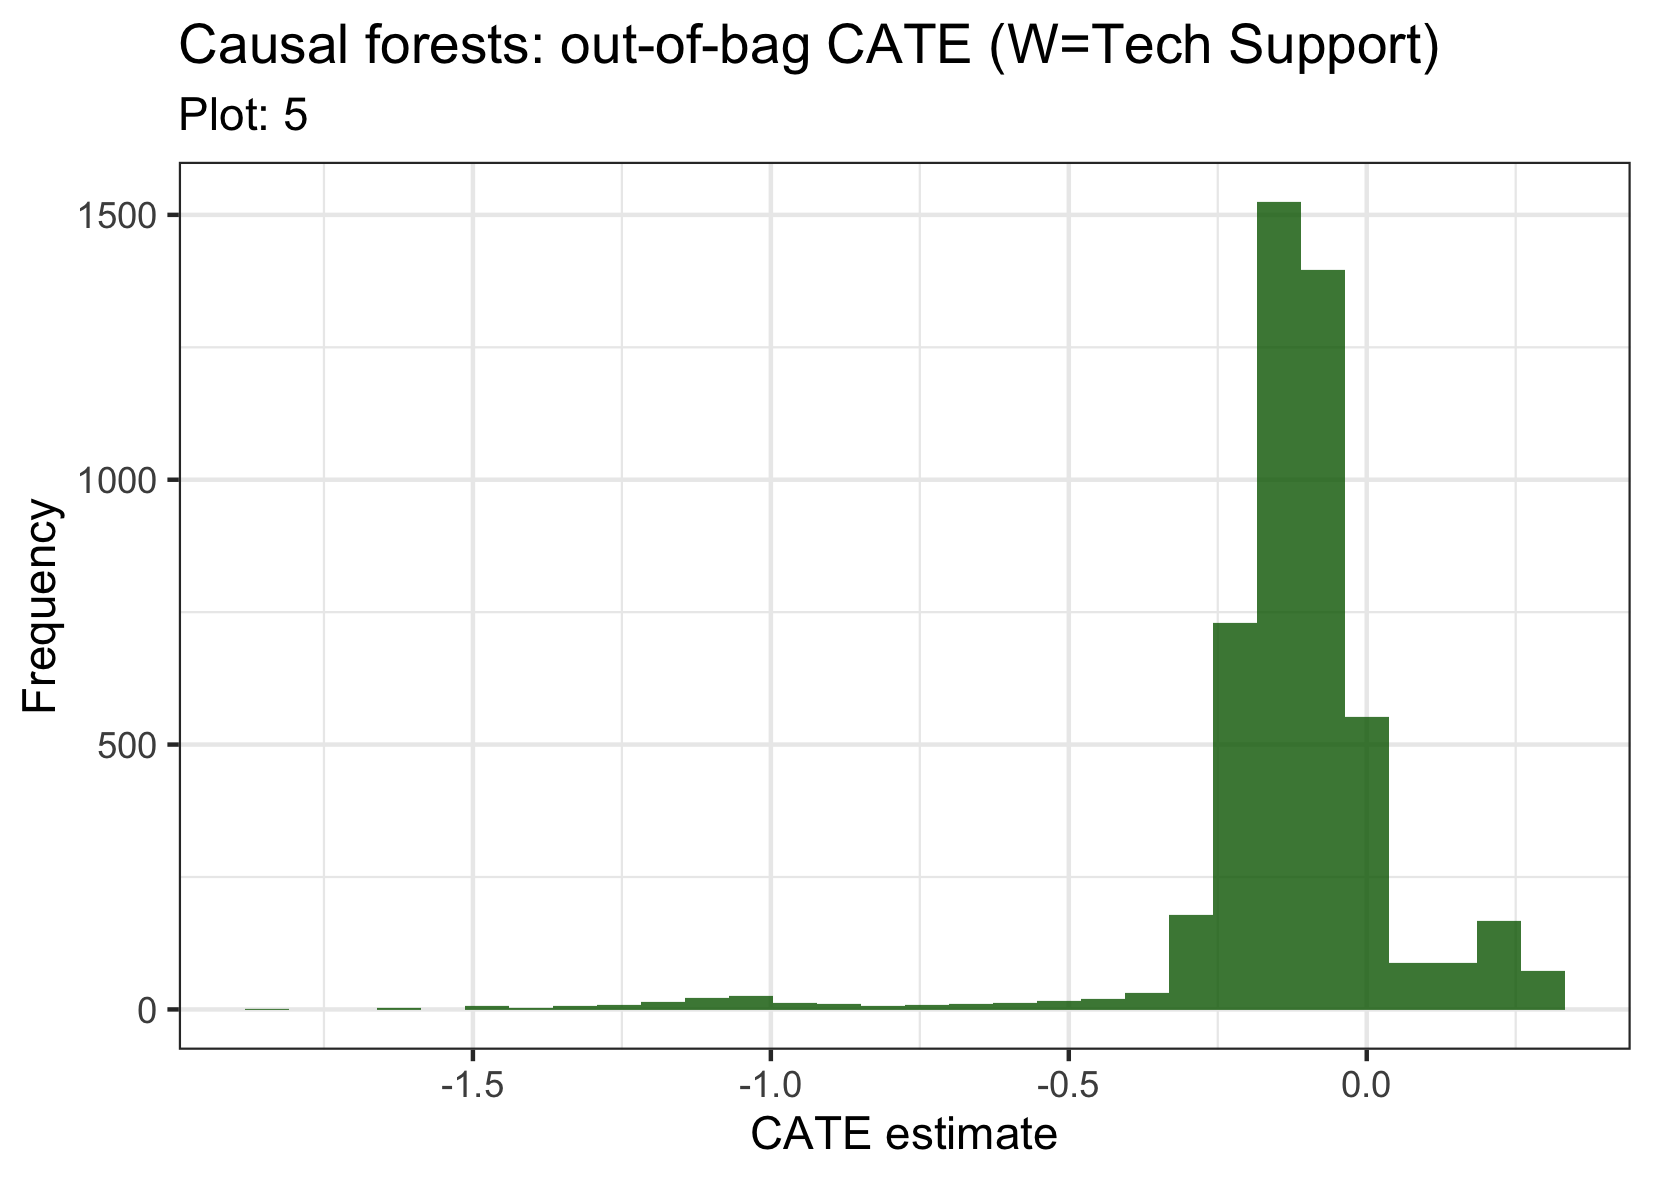
\includegraphics[scale=0.15]{chinchilab-template/chapters/appendices/ANALYSIS/CATE_5.png}
    \caption{Distribution of CATE (Model 5)}
    \label{fig:my_label}
\end{figure}

%%%%%%%%%%%%%%%%%%%%%%%%%%%%%%%%%%%%%%%%%%%%%%%%%%%%%%%%%%%%
\subsubsection{C.2.1.1 Nuisance Parameter Check}
%%%%%%%%%%%%%%%%%%%%%%%%%%%%%%%%%%%%%%%%%%%%%%%%%%%%%%%%%%%%
\begin{figure}[H]
    \centering
    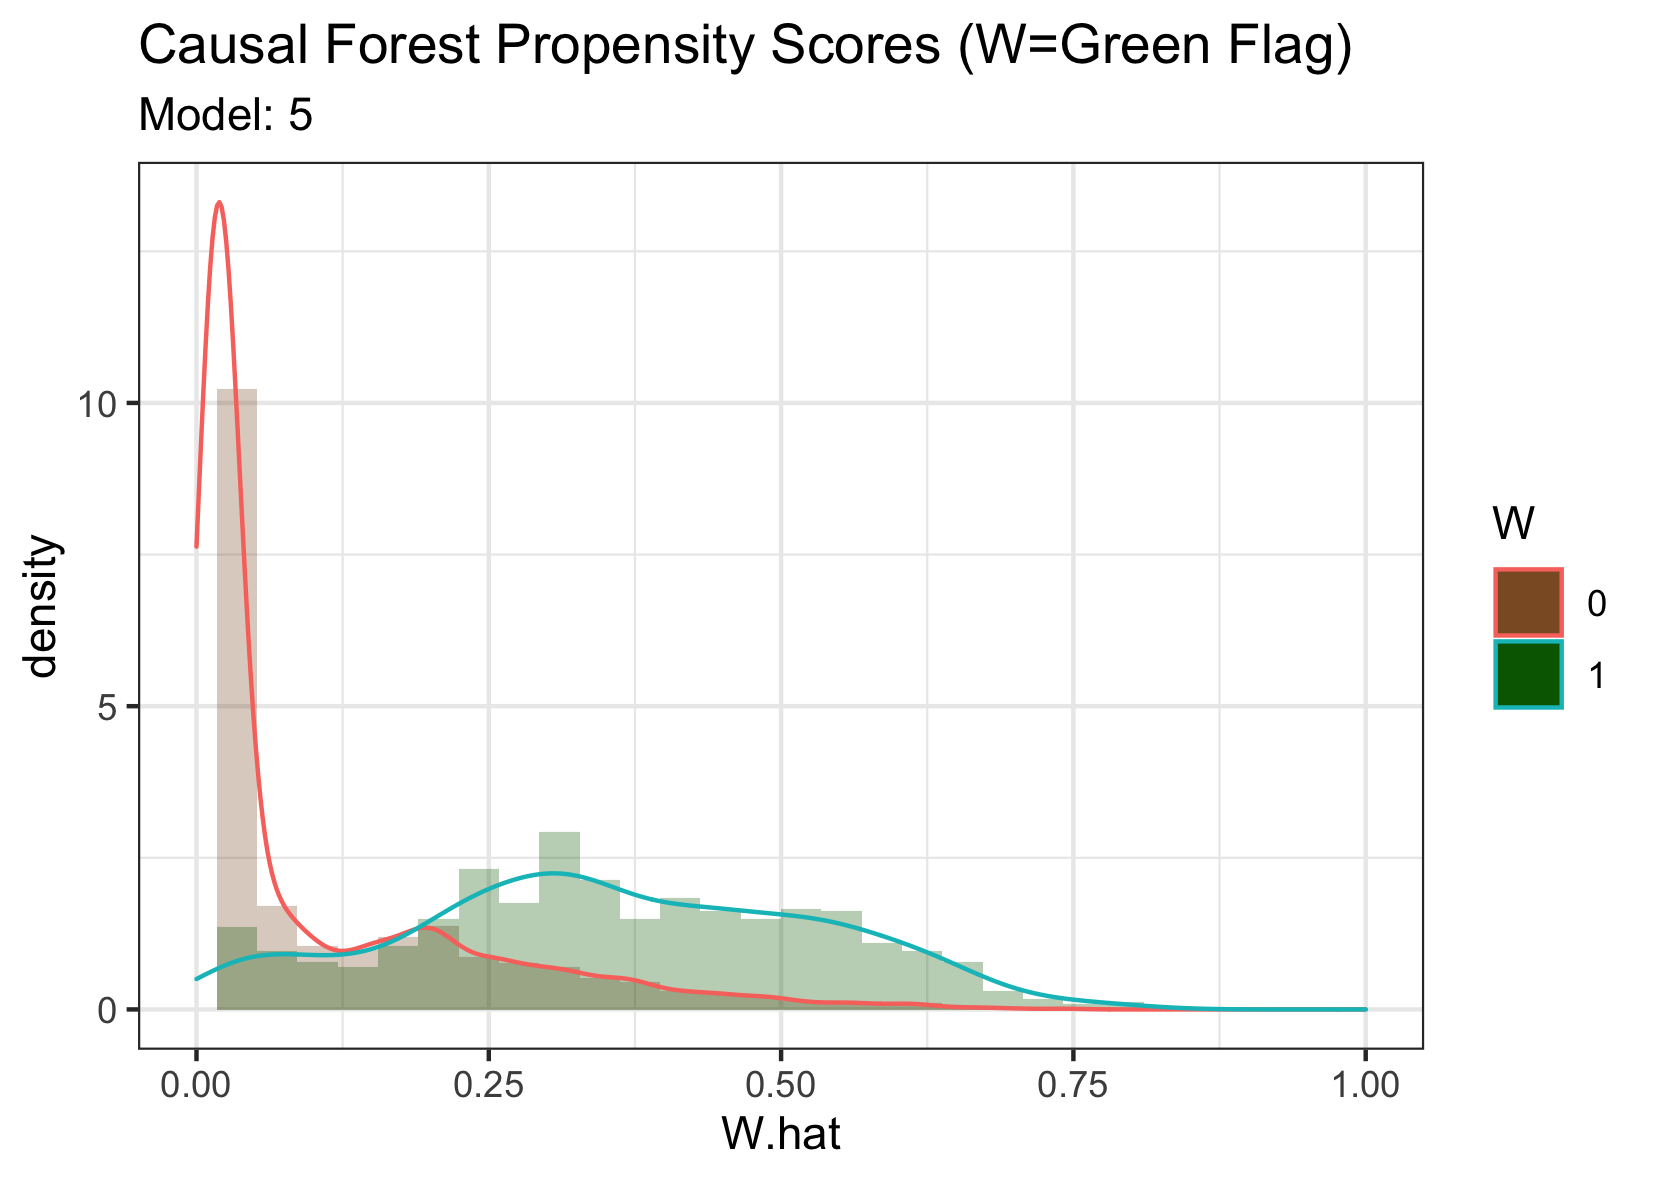
\includegraphics[scale=0.15]{chinchilab-template/chapters/appendices/ANALYSIS/prop_5.png}
    \caption{Propensity Score Distribution (Model 5)}
    \label{fig:my_label}
\end{figure}


\begin{table}[H]{
    \begin{subtable}{.5\textwidth}
    \centering
    \footnotesize
        {\begin{tabular}{@{\extracolsep{5pt}}lc} 
        \\[-1.8ex]\hline 
        \hline \\[-1.8ex] 
         & \multicolumn{1}{c}{\textit{Dependent variable: Green Flag}} \\ 
        \cline{2-2} 
        \\[-1.8ex] &   \\ 
        \hline \\[-1.8ex] 
         e.bar & 1.002$^{***}$ \\ 
          & (0.031) \\ 
          & \\ 
         e.residual & 1.117$^{***}$ \\ 
          & (0.036) \\ 
          & \\ 
        \hline \\[-1.8ex] 
        \hline 
        \hline \\[-1.8ex] 
        \textit{Note:}  & \multicolumn{1}{r}{$^{*}$p$<$0.1; $^{**}$p$<$0.05; $^{***}$p$<$0.01} \\ 
        \end{tabular}}
    \subcaption{Outcome Model}
    \end{subtable}
    \begin{subtable}{0.3\linewidth}
    \centering
    \footnotesize
        {\begin{tabular}{@{\extracolsep{5pt}}lc} 
        \\[-1.8ex]\hline 
        \hline \\[-1.8ex] 
         & \multicolumn{1}{c}{\textit{Dependent variable: Green Flag}} \\ 
        \cline{2-2} 
        \\[-1.8ex] &   \\ 
        \hline \\[-1.8ex] 
         m.bar & 1.001$^{***}$ \\ 
          & (0.011) \\ 
          & \\ 
         m.residual & 1.160$^{***}$ \\ 
          & (0.017) \\ 
          & \\ 
        \hline \\[-1.8ex] 
        \hline 
        \hline \\[-1.8ex] 
        \textit{Note:}  & \multicolumn{1}{r}{$^{*}$p$<$0.1; $^{**}$p$<$0.05; $^{***}$p$<$0.01} \\ 
        \end{tabular}}
    \subcaption{Propensity Model}
    \end{subtable}
\caption{Calibration Regressions (Model 5)}
\label{x}}
\end{table}


%%%%%%%%%%%%%%%%%%%%%%%%%%%%%%%%%%%%%%%%%%%%%%%%%%%%%%%%%%%%
\subsubsection{C.2.1.2 Heterogeneity Assessment}
%%%%%%%%%%%%%%%%%%%%%%%%%%%%%%%%%%%%%%%%%%%%%%%%%%%%%%%%%%%%

\begin{table}[h!]
\centering
\caption{Variable Importance (Model 5)}
\begin{tabular}{lr}
\\[-1.8ex]\hline 
\hline \\[-1.8ex] 
\rowcolor[HTML]{FFFFFF} 
{\color[HTML]{333333} \textbf{Covariate}} & {\color[HTML]{333333} \textbf{Value}} \\ \hline
\rowcolor[HTML]{FFFFFF} 
{\color[HTML]{333333} 2022} & \cellcolor[HTML]{00441B}{\color[HTML]{FFFFFF} 0.30362660} \\
\rowcolor[HTML]{FFFFFF} 
{\color[HTML]{333333} Issue Amount} & \cellcolor[HTML]{2B934B}{\color[HTML]{FFFFFF} 0.22873726} \\
\rowcolor[HTML]{FFFFFF} 
{\color[HTML]{333333} Time to Maturity (Days)} & \cellcolor[HTML]{6BBF71}{\color[HTML]{333333} 0.17635279} \\
\rowcolor[HTML]{FFFFFF} 
{\color[HTML]{333333} 2021} & \cellcolor[HTML]{F0F9ED}{\color[HTML]{333333} 0.05021639} \\
\rowcolor[HTML]{FFFFFF} 
{\color[HTML]{333333} 2020} & \cellcolor[HTML]{F3FBF1}{\color[HTML]{333333} 0.04394978} \\
\rowcolor[HTML]{FFFFFF} 
{\color[HTML]{333333} A} & \cellcolor[HTML]{F7FCF5}{\color[HTML]{333333} 0.03701316} \\ \hline
\end{tabular}
\end{table}

\begin{figure}[h!]
    \centering
    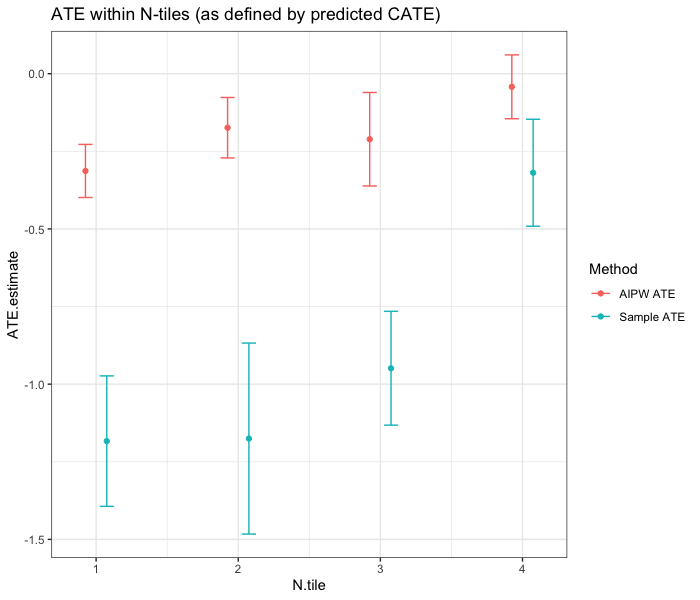
\includegraphics[scale=0.4]{chinchilab-template/chapters/appendices/ANALYSIS/ntile_cf2.png}
    \caption{Graph of ATE within Subgroups (Model 5)}
    \label{fig:my_label}
\end{figure}

\begin{figure}[H]
\centering
   \begin{subfigure}[b]{0.45\textwidth}
    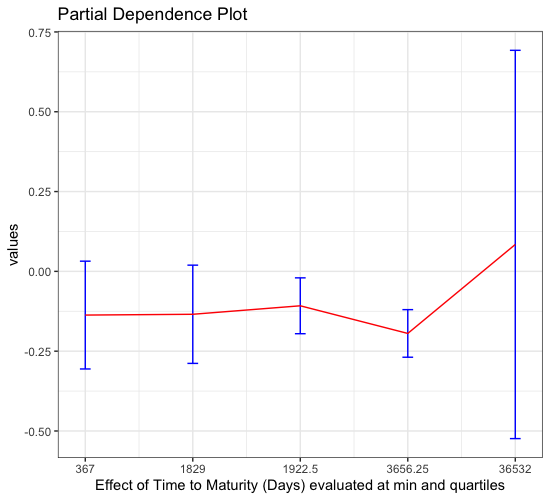
\includegraphics[width=0.9\textwidth]{chinchilab-template/chapters/appendices/ANALYSIS/PDP_cf2.png}
    \caption{Effect of Time to Maturity (Days)}
   \label{fig:Ng1} 
\end{subfigure}
\begin{subfigure}[b]{0.45\textwidth}
    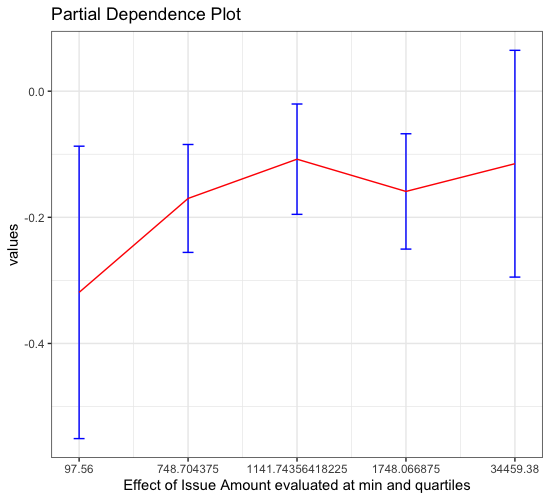
\includegraphics[width=0.9\textwidth]{chinchilab-template/chapters/appendices/ANALYSIS/PDP2_cf2.png}
    \caption{Effect of Issue Amount}
   \label{fig:Ng2}
\end{subfigure}
\\
\begin{subfigure}[b]{0.45\textwidth}
    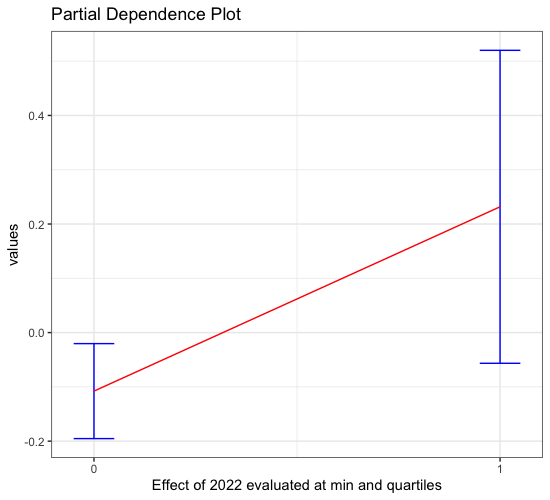
\includegraphics[width=0.9\textwidth]{chinchilab-template/chapters/appendices/ANALYSIS/PDP3_cf2.png}
    \caption{Effect of 2022}
   \label{fig:Ng2}
\end{subfigure}
\caption{Partial Dependency Plots (Model 5)}
\end{figure}

\begin{table}[H]
\caption{Heterogeneity across Covariates (Model 5)}
\label{Het}
\footnotesize
\begin{tabular}{lllll}
\\[-1.8ex]\hline 
\hline \\[-1.8ex] 
{\color[HTML]{333333} \textbf{Variable}} & {\color[HTML]{333333} \textbf{Mean ntile1}} & {\color[HTML]{333333} \textbf{Mean ntile2}} & {\color[HTML]{333333} \textbf{Mean ntile3}} & {\color[HTML]{333333} \textbf{Mean ntile4}} \\
\hline \\[-1.8ex] 
Time to   Maturity (Days) & \cellcolor[HTML]{78C78D}2910.99 & \cellcolor[HTML]{F3F9F8}2426.86 & \cellcolor[HTML]{FCFCFF}2390.91 & \cellcolor[HTML]{63BE7B}2992.96 \\
Issue Amount & \cellcolor[HTML]{FCFCFF}1160.36 & \cellcolor[HTML]{AEDDBC}1571.18 & \cellcolor[HTML]{63BE7B}1962.16 & \cellcolor[HTML]{97D3A8}1690.74 \\
Guarantor & \cellcolor[HTML]{E4F2EA}0.14 & \cellcolor[HTML]{DEF0E5}0.17 & \cellcolor[HTML]{E2F2E8}0.15 & \cellcolor[HTML]{CEEAD8}0.26 \\
2013 & \cellcolor[HTML]{EEF7F3}0.08 & \cellcolor[HTML]{EEF7F3}0.08 & \cellcolor[HTML]{F0F7F5}0.07 & \cellcolor[HTML]{F4F9F8}0.05 \\
2014 & \cellcolor[HTML]{ECF6F2}0.09 & \cellcolor[HTML]{EEF7F3}0.08 & \cellcolor[HTML]{F0F7F5}0.07 & \cellcolor[HTML]{F5FAF9}0.04 \\
2015 & \cellcolor[HTML]{E9F5EF}0.11 & \cellcolor[HTML]{EEF7F3}0.08 & \cellcolor[HTML]{F0F7F5}0.07 & \cellcolor[HTML]{F5FAF9}0.04 \\
2016 & \cellcolor[HTML]{E7F4ED}0.12 & \cellcolor[HTML]{EEF7F3}0.08 & \cellcolor[HTML]{F2F8F6}0.06 & \cellcolor[HTML]{F2F8F6}0.06 \\
2017 & \cellcolor[HTML]{ECF6F2}0.09 & \cellcolor[HTML]{ECF6F2}0.09 & \cellcolor[HTML]{EEF7F3}0.08 & \cellcolor[HTML]{F5FAF9}0.04 \\
2018 & \cellcolor[HTML]{F9FBFC}0.02 & \cellcolor[HTML]{F0F7F5}0.07 & \cellcolor[HTML]{E7F4ED}0.12 & \cellcolor[HTML]{F0F7F5}0.07 \\
2019 & \cellcolor[HTML]{E7F4ED}0.12 & \cellcolor[HTML]{E7F4ED}0.12 & \cellcolor[HTML]{F0F7F5}0.07 & \cellcolor[HTML]{FBFCFE}0.01 \\
2020 & \cellcolor[HTML]{FBFCFE}0.01 & \cellcolor[HTML]{F9FBFC}0.02 & \cellcolor[HTML]{ECF6F2}0.09 & \cellcolor[HTML]{E4F2EA}0.14 \\
2021 & \cellcolor[HTML]{FCFCFF}0 & \cellcolor[HTML]{F9FBFC}0.02 & \cellcolor[HTML]{ECF6F2}0.09 & \cellcolor[HTML]{E2F2E8}0.15 \\
2022 & \cellcolor[HTML]{FCFCFF}0 & \cellcolor[HTML]{FCFCFF}0 & \cellcolor[HTML]{FCFCFF}0 & \cellcolor[HTML]{CCE9D6}0.27 \\
Annual Coupon & \cellcolor[HTML]{63BE7B}0.86 & \cellcolor[HTML]{6EC385}0.8 & \cellcolor[HTML]{97D3A8}0.57 & \cellcolor[HTML]{B4DFC1}0.41 \\
Semi Annual   Coupon & \cellcolor[HTML]{E4F2EA}0.14 & \cellcolor[HTML]{D9EEE1}0.2 & \cellcolor[HTML]{B2DEBF}0.42 & \cellcolor[HTML]{94D2A5}0.59 \\
Quarterly & \cellcolor[HTML]{FCFCFF}0 & \cellcolor[HTML]{FCFCFF}0 & \cellcolor[HTML]{FCFCFF}0 & \cellcolor[HTML]{FCFCFF}0 \\
Senior   Secured Mortgage & \cellcolor[HTML]{E5F3EC}0.13 & \cellcolor[HTML]{E9F5EF}0.11 & \cellcolor[HTML]{EEF7F3}0.08 & \cellcolor[HTML]{F0F7F5}0.07 \\
Senior Secured & \cellcolor[HTML]{F0F7F5}0.07 & \cellcolor[HTML]{F4F9F8}0.05 & \cellcolor[HTML]{F5FAF9}0.04 & \cellcolor[HTML]{F2F8F6}0.06 \\
Senior Unsecured & \cellcolor[HTML]{8BCE9D}0.64 & \cellcolor[HTML]{8ED0A0}0.62 & \cellcolor[HTML]{8CCF9F}0.63 & \cellcolor[HTML]{79C78E}0.74 \\
Senior Non   Preferred & \cellcolor[HTML]{F9FBFC}0.02 & \cellcolor[HTML]{F9FBFC}0.02 & \cellcolor[HTML]{F2F8F6}0.06 & \cellcolor[HTML]{F7FAFB}0.03 \\
Senior Preferred & \cellcolor[HTML]{F4F9F8}0.05 & \cellcolor[HTML]{F2F8F6}0.06 & \cellcolor[HTML]{F2F8F6}0.06 & \cellcolor[HTML]{F4F9F8}0.05 \\
Senior   Subordinated Unsecured & \cellcolor[HTML]{FBFCFE}0.01 & \cellcolor[HTML]{FCFCFF}0 & \cellcolor[HTML]{FCFCFF}0 & \cellcolor[HTML]{FCFCFF}0 \\
Subordinated   Unsecured & \cellcolor[HTML]{F7FAFB}0.03 & \cellcolor[HTML]{F7FAFB}0.03 & \cellcolor[HTML]{FBFCFE}0.01 & \cellcolor[HTML]{FBFCFE}0.01 \\
Basic Materials & \cellcolor[HTML]{FBFCFE}0.01 & \cellcolor[HTML]{FCFCFF}0 & \cellcolor[HTML]{FCFCFF}0 & \cellcolor[HTML]{FBFCFE}0.01 \\
Consumer   Cyclicals & \cellcolor[HTML]{FBFCFE}0.01 & \cellcolor[HTML]{FCFCFF}0 & \cellcolor[HTML]{FCFCFF}0 & \cellcolor[HTML]{FCFCFF}0 \\
Consumer   Non Cyclicals & \cellcolor[HTML]{FCFCFF}0 & \cellcolor[HTML]{FCFCFF}0 & \cellcolor[HTML]{FCFCFF}0 & \cellcolor[HTML]{FCFCFF}0 \\
Energy & \cellcolor[HTML]{FBFCFE}0.01 & \cellcolor[HTML]{FBFCFE}0.01 & \cellcolor[HTML]{FCFCFF}0 & \cellcolor[HTML]{FCFCFF}0 \\
Financials & \cellcolor[HTML]{80CA94}0.7 & \cellcolor[HTML]{84CB97}0.68 & \cellcolor[HTML]{82CB96}0.69 & \cellcolor[HTML]{80CA94}0.7 \\
Healthcare & \cellcolor[HTML]{FCFCFF}0 & \cellcolor[HTML]{FCFCFF}0 & \cellcolor[HTML]{FCFCFF}0 & \cellcolor[HTML]{FCFCFF}0 \\
Industrials & \cellcolor[HTML]{F9FBFC}0.02 & \cellcolor[HTML]{FBFCFE}0.01 & \cellcolor[HTML]{FBFCFE}0.01 & \cellcolor[HTML]{FBFCFE}0.01 \\
Institutions,   Associations \& Organizations & \cellcolor[HTML]{F9FBFC}0.02 & \cellcolor[HTML]{F7FAFB}0.03 & \cellcolor[HTML]{F0F7F5}0.07 & \cellcolor[HTML]{F5FAF9}0.04 \\
Real Estate & \cellcolor[HTML]{FCFCFF}0 & \cellcolor[HTML]{FCFCFF}0 & \cellcolor[HTML]{FCFCFF}0 & \cellcolor[HTML]{FCFCFF}0 \\
Technology & \cellcolor[HTML]{FBFCFE}0.01 & \cellcolor[HTML]{FBFCFE}0.01 & \cellcolor[HTML]{FBFCFE}0.01 & \cellcolor[HTML]{FCFCFF}0 \\
Utilities & \cellcolor[HTML]{F7FAFB}0.03 & \cellcolor[HTML]{F9FBFC}0.02 & \cellcolor[HTML]{FBFCFE}0.01 & \cellcolor[HTML]{FBFCFE}0.01 \\
AAA & \cellcolor[HTML]{C0E4CB}0.34 & \cellcolor[HTML]{AEDDBC}0.44 & \cellcolor[HTML]{A4D8B3}0.5 & \cellcolor[HTML]{A7DAB6}0.48 \\
AA & \cellcolor[HTML]{CBE8D5}0.28 & \cellcolor[HTML]{D7EDDF}0.21 & \cellcolor[HTML]{DBEFE2}0.19 & \cellcolor[HTML]{C5E6D0}0.31 \\
A & \cellcolor[HTML]{D2EBDB}0.24 & \cellcolor[HTML]{E0F1E7}0.16 & \cellcolor[HTML]{EBF5F0}0.1 & \cellcolor[HTML]{E9F5EF}0.11 \\
BBB & \cellcolor[HTML]{E7F4ED}0.12 & \cellcolor[HTML]{DEF0E5}0.17 & \cellcolor[HTML]{D9EEE1}0.2 & \cellcolor[HTML]{ECF6F2}0.09 \\
BB & \cellcolor[HTML]{F9FBFC}0.02 & \cellcolor[HTML]{F9FBFC}0.02 & \cellcolor[HTML]{FBFCFE}0.01 & \cellcolor[HTML]{FBFCFE}0.01 \\
EUR & \cellcolor[HTML]{6BC182}0.82 & \cellcolor[HTML]{7CC991}0.72 & \cellcolor[HTML]{A2D8B1}0.51 & \cellcolor[HTML]{B7E0C4}0.39 \\
\hline \\[-1.8ex] 
\end{tabular}
\end{table}

\newpage

%%%%%%%%%%%%%%%%%%%%%%%%%%%%%%%%%%%%%%%%%%%%%%%%%%%%%%%%%%%%
\subsection{C.2.2 With Issuer Controls}
%%%%%%%%%%%%%%%%%%%%%%%%%%%%%%%%%%%%%%%%%%%%%%%%%%%%%%%%%%%%

\begin{figure}[H]
    \centering
    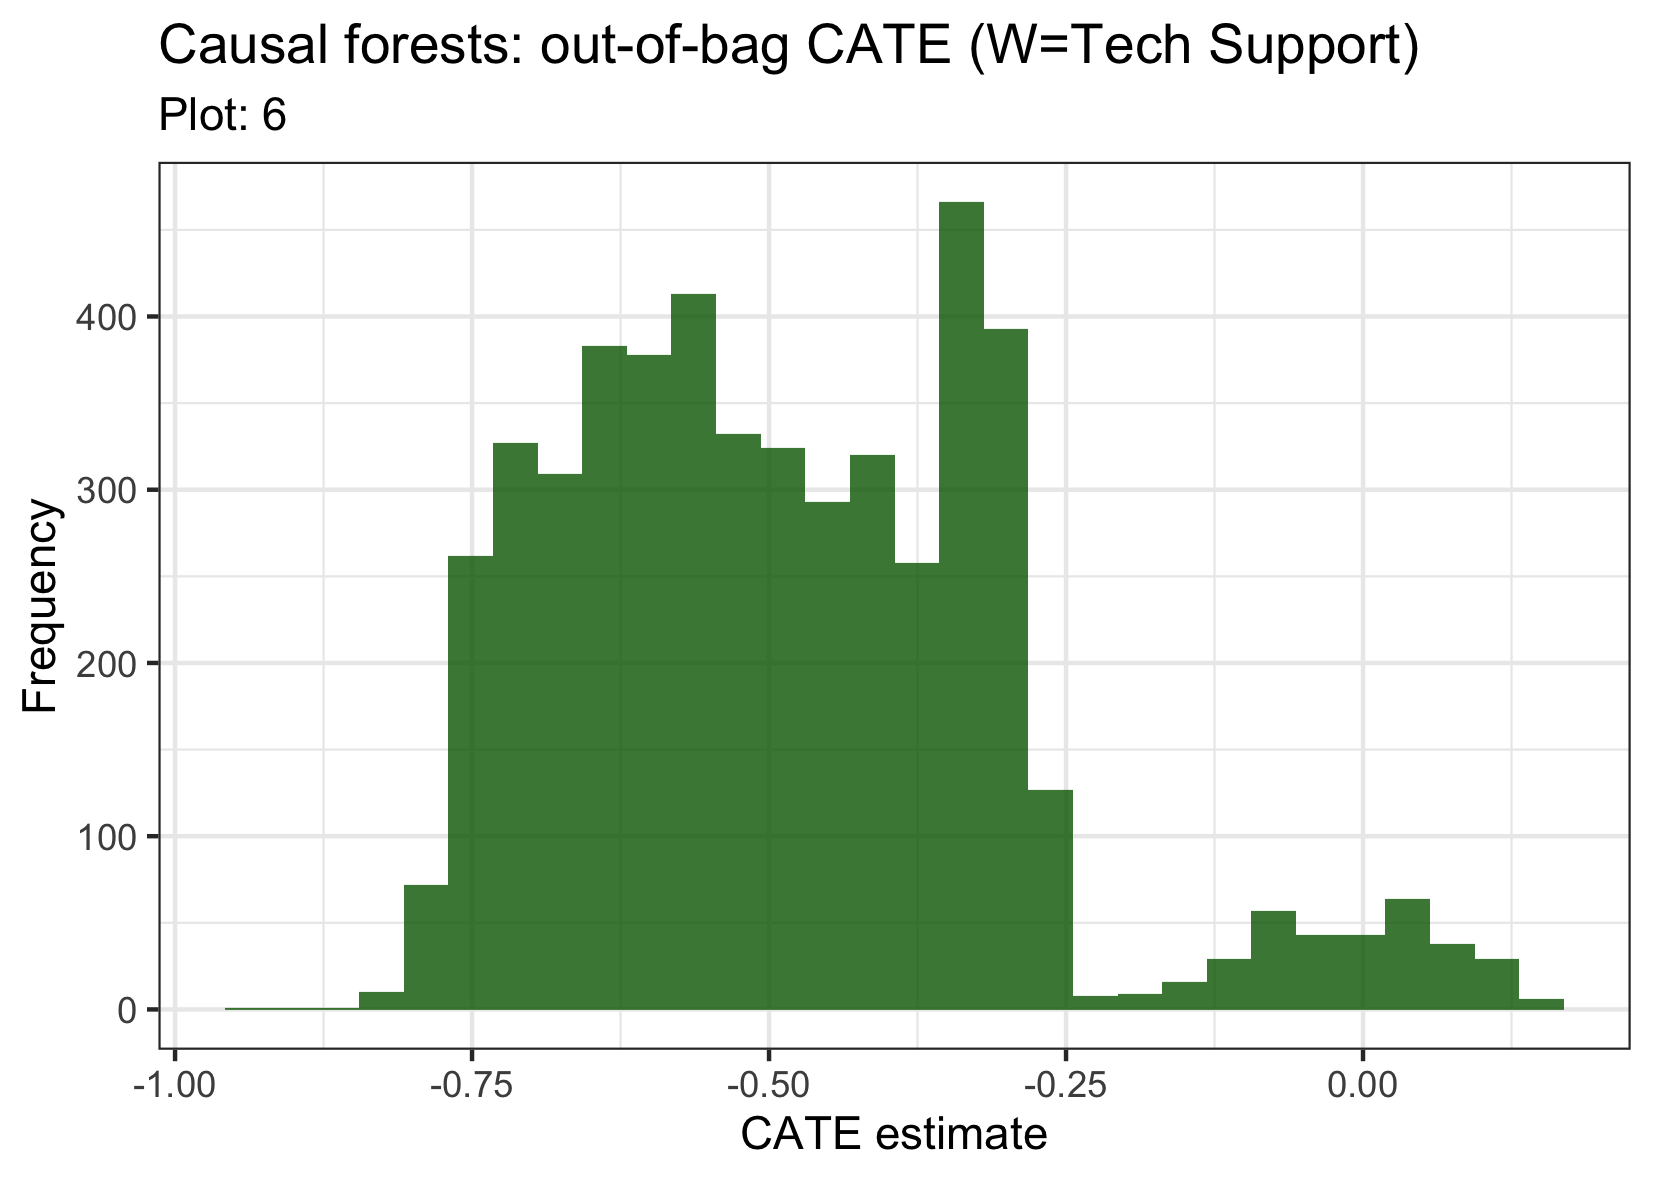
\includegraphics[scale=0.15]{chinchilab-template/chapters/appendices/ANALYSIS/CATE_6.png}
    \caption{Distribution of CATE (Model 6)}
    \label{fig:my_label}
\end{figure}

%%%%%%%%%%%%%%%%%%%%%%%%%%%%%%%%%%%%%%%%%%%%%%%%%%%%%%%%%%%%
\subsubsection{C.2.2.1 Nuisance Parameter Check}
%%%%%%%%%%%%%%%%%%%%%%%%%%%%%%%%%%%%%%%%%%%%%%%%%%%%%%%%%%%%
\begin{figure}[H]
    \centering
    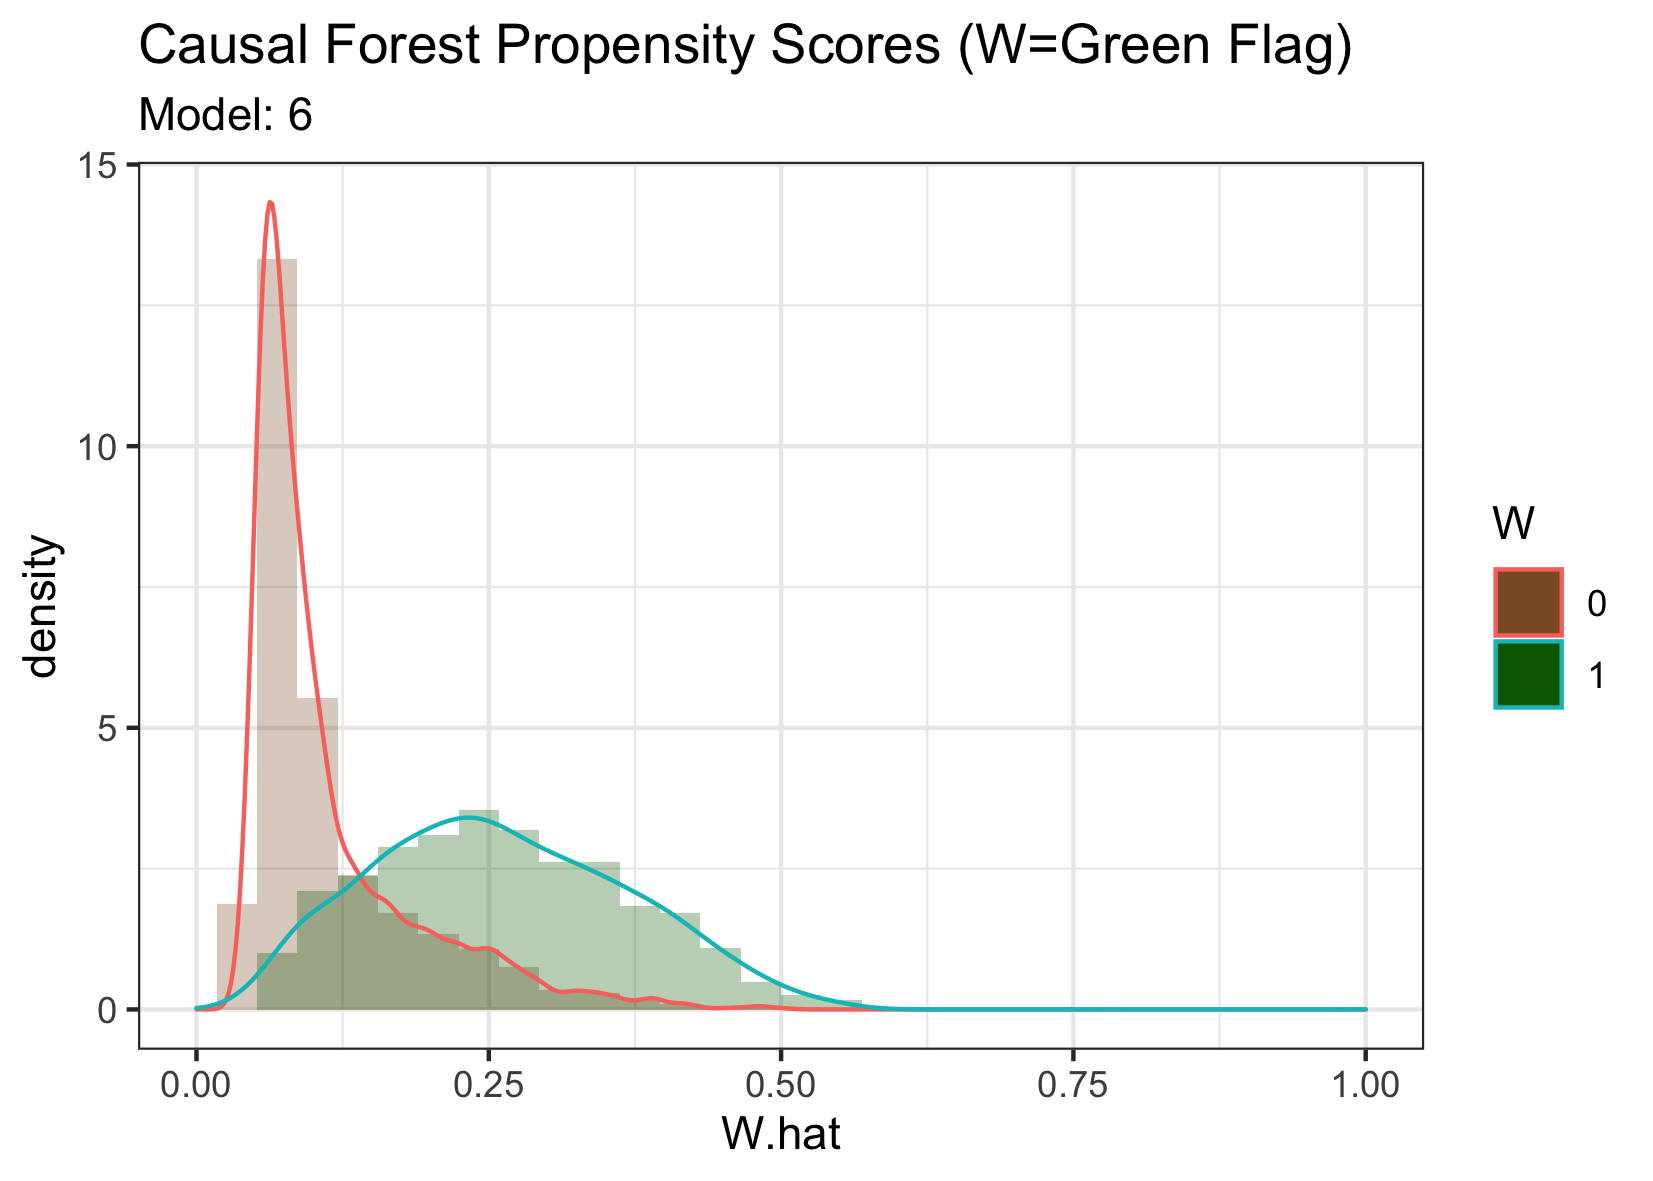
\includegraphics[scale=0.15]{chinchilab-template/chapters/appendices/ANALYSIS/prop_6.png}
    \caption{Propensity Score Distribution (Model 6)}
    \label{fig:my_label}
\end{figure}


\begin{table}[H]{
    \begin{subtable}{.5\textwidth}
    \centering
    \scriptsize
        {\begin{tabular}{@{\extracolsep{5pt}}lc} 
        \\[-1.8ex]\hline 
        \hline \\[-1.8ex] 
         & \multicolumn{1}{c}{\textit{Dependent variable: Green Flag}} \\ 
        \cline{2-2} 
        \\[-1.8ex] &   \\ 
        \hline \\[-1.8ex] 
         e.bar & 1.003$^{***}$ \\ 
          & (0.031) \\ 
          & \\ 
         e.residual & 1.946$^{***}$ \\ 
          & (0.061) \\ 
          & \\ 
        \hline \\[-1.8ex] 
        \hline 
        \hline \\[-1.8ex] 
        \textit{Note:}  & \multicolumn{1}{r}{$^{*}$p$<$0.1; $^{**}$p$<$0.05; $^{***}$p$<$0.01} \\ 
        \end{tabular} }
    \subcaption{Outcome Model}
    \end{subtable}
    \begin{subtable}{0.3\linewidth}
    \centering
    \scriptsize
        {\begin{tabular}{@{\extracolsep{5pt}}lc} 
        \\[-1.8ex]\hline 
        \hline \\[-1.8ex] 
         & \multicolumn{1}{c}{\textit{Dependent variable: Green Flag}} \\ 
        \cline{2-2} 
        \\[-1.8ex] &   \\ 
        \hline \\[-1.8ex] 
         m.bar & 1.000$^{***}$ \\ 
          & (0.012) \\ 
          & \\ 
         m.residual & 2.056$^{***}$ \\ 
          & (0.039) \\ 
          & \\ 
        \hline \\[-1.8ex] 
        \hline 
        \hline \\[-1.8ex] 
        \textit{Note:}  & \multicolumn{1}{r}{$^{*}$p$<$0.1; $^{**}$p$<$0.05; $^{***}$p$<$0.01} \\ 
        \end{tabular} }
    \subcaption{Propensity Model}
    \end{subtable}
\caption{Calibration Regressions (Model 6)}
\label{x}}
\end{table}



\newpage

%%%%%%%%%%%%%%%%%%%%%%%%%%%%%%%%%%%%%%%%%%%%%%%%%%%%%%%%%%%%
\subsubsection{C.2.2.2 Heterogeneity Assessment}
%%%%%%%%%%%%%%%%%%%%%%%%%%%%%%%%%%%%%%%%%%%%%%%%%%%%%%%%%%%%

\begin{table}[h!]
\centering
\caption{Variable Importance (Model 6)}
\begin{tabular}{lr}
\\[-1.8ex]\hline 
\hline \\[-1.8ex] 
\rowcolor[HTML]{FFFFFF} 
{\color[HTML]{333333} \textbf{Covariate}} & {\color[HTML]{333333} \textbf{Value}} \\ \hline
\rowcolor[HTML]{FFFFFF} 
{\color[HTML]{333333} 2022} & \cellcolor[HTML]{00441B}{\color[HTML]{FFFFFF} 0.11191270} \\
\rowcolor[HTML]{FFFFFF} 
{\color[HTML]{333333} Issue Amount} & \cellcolor[HTML]{117936}{\color[HTML]{FFFFFF} 0.10161593} \\
\rowcolor[HTML]{FFFFFF} 
{\color[HTML]{333333} Time to Maturity (Days)} & \cellcolor[HTML]{2C944C}{\color[HTML]{FFFFFF} 0.09521301} \\
\rowcolor[HTML]{FFFFFF} 
{\color[HTML]{333333} EUR} & \cellcolor[HTML]{D9F0D3}{\color[HTML]{333333} 0.06385172} \\
\rowcolor[HTML]{FFFFFF} 
{\color[HTML]{333333} Annual Coupon} & \cellcolor[HTML]{E5F5E1}{\color[HTML]{333333} 0.06081552} \\
\rowcolor[HTML]{FFFFFF} 
{\color[HTML]{333333} Semi Annual Coupon} & \cellcolor[HTML]{F7FCF5}{\color[HTML]{333333} 0.05372767} \\ \hline
\end{tabular}
\end{table}

\begin{figure}[h!]
    \centering
    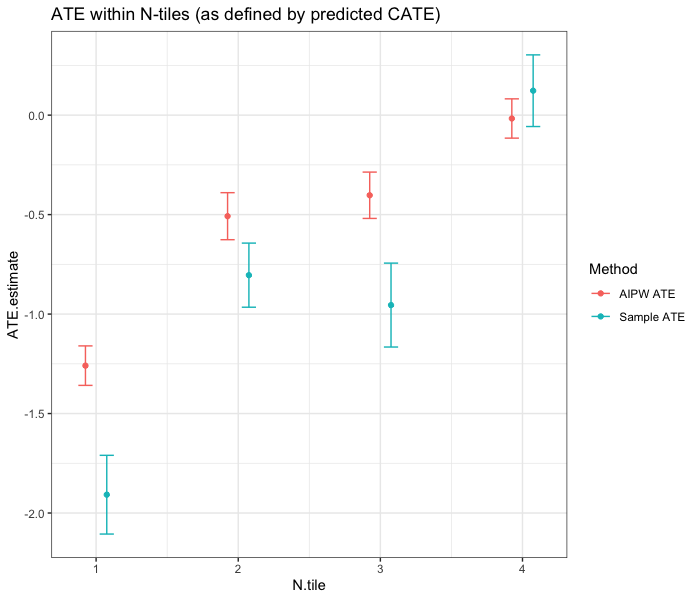
\includegraphics[scale=0.5]{chinchilab-template/chapters/appendices/ANALYSIS/ntile_cf2.1.png}
    \caption{Graph of ATE within Subgroups (Model 6)}
    \label{fig:my_label}
\end{figure}

\begin{figure}[H]
\centering
   \begin{subfigure}[b]{0.45\textwidth}
    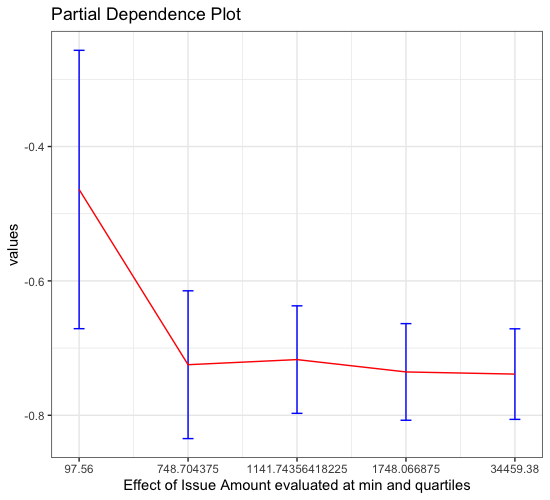
\includegraphics[width=0.9\textwidth]{chinchilab-template/chapters/appendices/ANALYSIS/PDP_cf2.1.png}
    \caption{Effect of Issue Amount}
   \label{fig:Ng1} 
\end{subfigure}
\begin{subfigure}[b]{0.45\textwidth}
    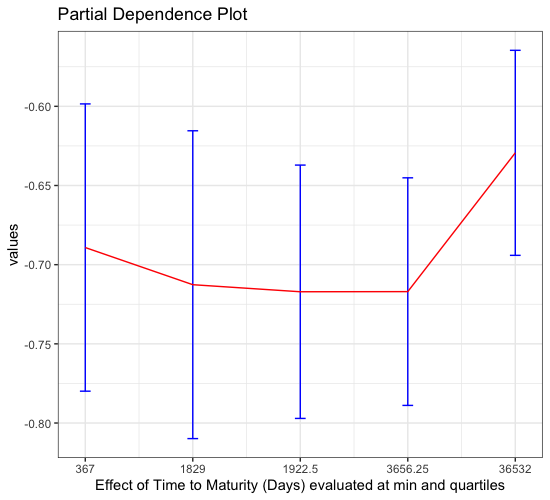
\includegraphics[width=0.9\textwidth]{chinchilab-template/chapters/appendices/ANALYSIS/PDP2_cf2.1.png}
    \caption{Effect of Time to Maturity (Days)}
   \label{fig:Ng2}
\end{subfigure}
\\
\begin{subfigure}[b]{0.45\textwidth}
    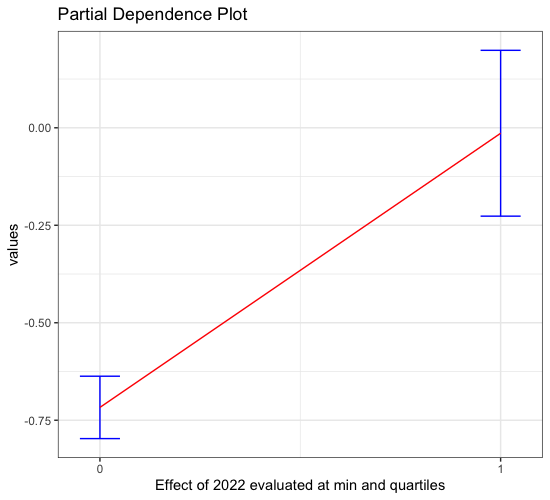
\includegraphics[width=0.9\textwidth]{chinchilab-template/chapters/appendices/ANALYSIS/PDP3_cf2.1.png}
    \caption{Effect of 2022}
   \label{fig:Ng2}
\end{subfigure}
\caption{Partial Dependency Plots (Model 6)}
\end{figure}

\begin{table}[H]
\caption{Heterogeneity across Covariates (Model 6)}
\label{Het}
\footnotesize
\begin{tabular}{lllll}
\\[-1.8ex]\hline 
\hline \\[-1.8ex] 
{\color[HTML]{333333} \textbf{Variable}} & {\color[HTML]{333333} \textbf{Mean ntile1}} & {\color[HTML]{333333} \textbf{Mean ntile2}} & {\color[HTML]{333333} \textbf{Mean ntile3}} & {\color[HTML]{333333} \textbf{Mean ntile4}} \\
\hline \\[-1.8ex] 
Time to   Maturity (Days) & \cellcolor[HTML]{A7DAB6}2742.93 & \cellcolor[HTML]{63BE7B}3504.99 & \cellcolor[HTML]{ADDCBB}2683.71 & \cellcolor[HTML]{FCFCFF}1790.09 \\
Issue Amount & \cellcolor[HTML]{63BE7B}1766.86 & \cellcolor[HTML]{8FD0A1}1622.31 & \cellcolor[HTML]{FCFCFF}1261 & \cellcolor[HTML]{6DC284}1734.27 \\
Guarantor & \cellcolor[HTML]{DFF1E6}0.19 & \cellcolor[HTML]{DFF1E6}0.19 & \cellcolor[HTML]{ECF6F1}0.11 & \cellcolor[HTML]{D8EEE0}0.24 \\
2013 & \cellcolor[HTML]{EAF5F0}0.12 & \cellcolor[HTML]{F5F9F9}0.05 & \cellcolor[HTML]{F5F9F9}0.05 & \cellcolor[HTML]{F3F9F8}0.06 \\
2014 & \cellcolor[HTML]{ECF6F1}0.11 & \cellcolor[HTML]{F3F9F8}0.06 & \cellcolor[HTML]{F3F9F8}0.06 & \cellcolor[HTML]{F5F9F9}0.05 \\
2015 & \cellcolor[HTML]{F3F9F8}0.06 & \cellcolor[HTML]{EFF7F4}0.09 & \cellcolor[HTML]{EFF7F4}0.09 & \cellcolor[HTML]{F2F8F6}0.07 \\
2016 & \cellcolor[HTML]{F2F8F6}0.07 & \cellcolor[HTML]{EFF7F4}0.09 & \cellcolor[HTML]{F0F8F5}0.08 & \cellcolor[HTML]{F0F8F5}0.08 \\
2017 & \cellcolor[HTML]{F9FBFD}0.02 & \cellcolor[HTML]{EDF6F2}0.1 & \cellcolor[HTML]{ECF6F1}0.11 & \cellcolor[HTML]{F3F9F8}0.06 \\
2018 & \cellcolor[HTML]{FBFCFE}0.01 & \cellcolor[HTML]{EDF6F2}0.1 & \cellcolor[HTML]{ECF6F1}0.11 & \cellcolor[HTML]{F3F9F8}0.06 \\
2019 & \cellcolor[HTML]{F9FBFD}0.02 & \cellcolor[HTML]{E7F4ED}0.14 & \cellcolor[HTML]{E9F4EE}0.13 & \cellcolor[HTML]{F8FBFC}0.03 \\
2020 & \cellcolor[HTML]{FBFCFE}0.01 & \cellcolor[HTML]{F0F8F5}0.08 & \cellcolor[HTML]{EFF7F4}0.09 & \cellcolor[HTML]{F2F8F6}0.07 \\
2021 & \cellcolor[HTML]{F8FBFC}0.03 & \cellcolor[HTML]{F0F8F5}0.08 & \cellcolor[HTML]{F0F8F5}0.08 & \cellcolor[HTML]{F2F8F6}0.07 \\
2022 & \cellcolor[HTML]{FCFCFF}0 & \cellcolor[HTML]{FCFCFF}0 & \cellcolor[HTML]{FCFCFF}0 & \cellcolor[HTML]{D3ECDC}0.27 \\
Annual Coupon & \cellcolor[HTML]{63BE7B}1 & \cellcolor[HTML]{6AC181}0.96 & \cellcolor[HTML]{B3DFC0}0.48 & \cellcolor[HTML]{DEF0E5}0.2 \\
Semi Annual   Coupon & \cellcolor[HTML]{FCFCFF}0 & \cellcolor[HTML]{F6FAFA}0.04 & \cellcolor[HTML]{AEDDBC}0.51 & \cellcolor[HTML]{82CB96}0.8 \\
Quarterly & \cellcolor[HTML]{FCFCFF}0 & \cellcolor[HTML]{FCFCFF}0 & \cellcolor[HTML]{FCFCFF}0 & \cellcolor[HTML]{FCFCFF}0 \\
Senior   Secured Mortgage & \cellcolor[HTML]{FCFCFF}0 & \cellcolor[HTML]{DFF1E6}0.19 & \cellcolor[HTML]{E7F4ED}0.14 & \cellcolor[HTML]{F5F9F9}0.05 \\
Senior Secured & \cellcolor[HTML]{F8FBFC}0.03 & \cellcolor[HTML]{F0F8F5}0.08 & \cellcolor[HTML]{F8FBFC}0.03 & \cellcolor[HTML]{F2F8F6}0.07 \\
Senior Unsecured & \cellcolor[HTML]{7CC891}0.84 & \cellcolor[HTML]{A8DAB7}0.55 & \cellcolor[HTML]{ADDCBB}0.52 & \cellcolor[HTML]{8DCF9F}0.73 \\
Senior Non   Preferred & \cellcolor[HTML]{FCFCFF}0 & \cellcolor[HTML]{F9FBFD}0.02 & \cellcolor[HTML]{EFF7F4}0.09 & \cellcolor[HTML]{F9FBFD}0.02 \\
Senior Preferred & \cellcolor[HTML]{FCFCFF}0 & \cellcolor[HTML]{F6FAFA}0.04 & \cellcolor[HTML]{E9F4EE}0.13 & \cellcolor[HTML]{F6FAFA}0.04 \\
Senior   Subordinated Unsecured & \cellcolor[HTML]{FBFCFE}0.01 & \cellcolor[HTML]{FCFCFF}0 & \cellcolor[HTML]{FCFCFF}0 & \cellcolor[HTML]{FCFCFF}0 \\
Subordinated   Unsecured & \cellcolor[HTML]{FBFCFE}0.01 & \cellcolor[HTML]{F9FBFD}0.02 & \cellcolor[HTML]{F5F9F9}0.05 & \cellcolor[HTML]{FCFCFF}0 \\
Basic Materials & \cellcolor[HTML]{F9FBFD}0.02 & \cellcolor[HTML]{FCFCFF}0 & \cellcolor[HTML]{FCFCFF}0 & \cellcolor[HTML]{FCFCFF}0 \\
Consumer   Cyclicals & \cellcolor[HTML]{F9FBFD}0.02 & \cellcolor[HTML]{FCFCFF}0 & \cellcolor[HTML]{FCFCFF}0 & \cellcolor[HTML]{FCFCFF}0 \\
Consumer   Non Cyclicals & \cellcolor[HTML]{FCFCFF}0 & \cellcolor[HTML]{FCFCFF}0 & \cellcolor[HTML]{FCFCFF}0 & \cellcolor[HTML]{FCFCFF}0 \\
Energy & \cellcolor[HTML]{F9FBFD}0.02 & \cellcolor[HTML]{FCFCFF}0 & \cellcolor[HTML]{FCFCFF}0 & \cellcolor[HTML]{FCFCFF}0 \\
Financials & \cellcolor[HTML]{A8DAB7}0.55 & \cellcolor[HTML]{9BD5AB}0.64 & \cellcolor[HTML]{88CD9B}0.76 & \cellcolor[HTML]{7FCA93}0.82 \\
Healthcare & \cellcolor[HTML]{FCFCFF}0 & \cellcolor[HTML]{FCFCFF}0 & \cellcolor[HTML]{FCFCFF}0 & \cellcolor[HTML]{FCFCFF}0 \\
Industrials & \cellcolor[HTML]{FBFCFE}0.01 & \cellcolor[HTML]{F9FBFD}0.02 & \cellcolor[HTML]{FBFCFE}0.01 & \cellcolor[HTML]{FCFCFF}0 \\
Institutions,   Associations \& Organizations & \cellcolor[HTML]{F9FBFD}0.02 & \cellcolor[HTML]{F9FBFD}0.02 & \cellcolor[HTML]{F2F8F6}0.07 & \cellcolor[HTML]{F6FAFA}0.04 \\
Real Estate & \cellcolor[HTML]{FCFCFF}0 & \cellcolor[HTML]{FBFCFE}0.01 & \cellcolor[HTML]{FCFCFF}0 & \cellcolor[HTML]{FCFCFF}0 \\
Technology & \cellcolor[HTML]{F9FBFD}0.02 & \cellcolor[HTML]{FCFCFF}0 & \cellcolor[HTML]{FCFCFF}0 & \cellcolor[HTML]{FCFCFF}0 \\
Utilities & \cellcolor[HTML]{F6FAFA}0.04 & \cellcolor[HTML]{F9FBFD}0.02 & \cellcolor[HTML]{FBFCFE}0.01 & \cellcolor[HTML]{FCFCFF}0 \\
AAA & \cellcolor[HTML]{CDE9D7}0.31 & \cellcolor[HTML]{B3DFC0}0.48 & \cellcolor[HTML]{CAE8D4}0.33 & \cellcolor[HTML]{9CD5AC}0.63 \\
AA & \cellcolor[HTML]{D2EBDB}0.28 & \cellcolor[HTML]{D3ECDC}0.27 & \cellcolor[HTML]{DEF0E5}0.2 & \cellcolor[HTML]{D6EDDE}0.25 \\
A & \cellcolor[HTML]{DCEFE4}0.21 & \cellcolor[HTML]{ECF6F1}0.11 & \cellcolor[HTML]{DCEFE4}0.21 & \cellcolor[HTML]{F0F8F5}0.08 \\
BBB & \cellcolor[HTML]{DFF1E6}0.19 & \cellcolor[HTML]{E9F4EE}0.13 & \cellcolor[HTML]{D9EEE1}0.23 & \cellcolor[HTML]{F6FAFA}0.04 \\
BB & \cellcolor[HTML]{F9FBFD}0.02 & \cellcolor[HTML]{FCFCFF}0 & \cellcolor[HTML]{F9FBFD}0.02 & \cellcolor[HTML]{FCFCFF}0 \\
EUR & \cellcolor[HTML]{63BE7B}1 & \cellcolor[HTML]{77C78D}0.87 & \cellcolor[HTML]{C1E4CC}0.39 & \cellcolor[HTML]{DFF1E6}0.19 \\
\hline \\[-1.8ex] 
\end{tabular}
\end{table}

\newpage

%%%%%%%%%%%%%%%%%%%%%%%%%%%%%%%%%%%%%%%%%%%%%%%%%%%%%%%%%%%%
\subsection{C.2.3 PSM Sample}
%%%%%%%%%%%%%%%%%%%%%%%%%%%%%%%%%%%%%%%%%%%%%%%%%%%%%%%%%%%%

\begin{figure}[H]
    \centering
    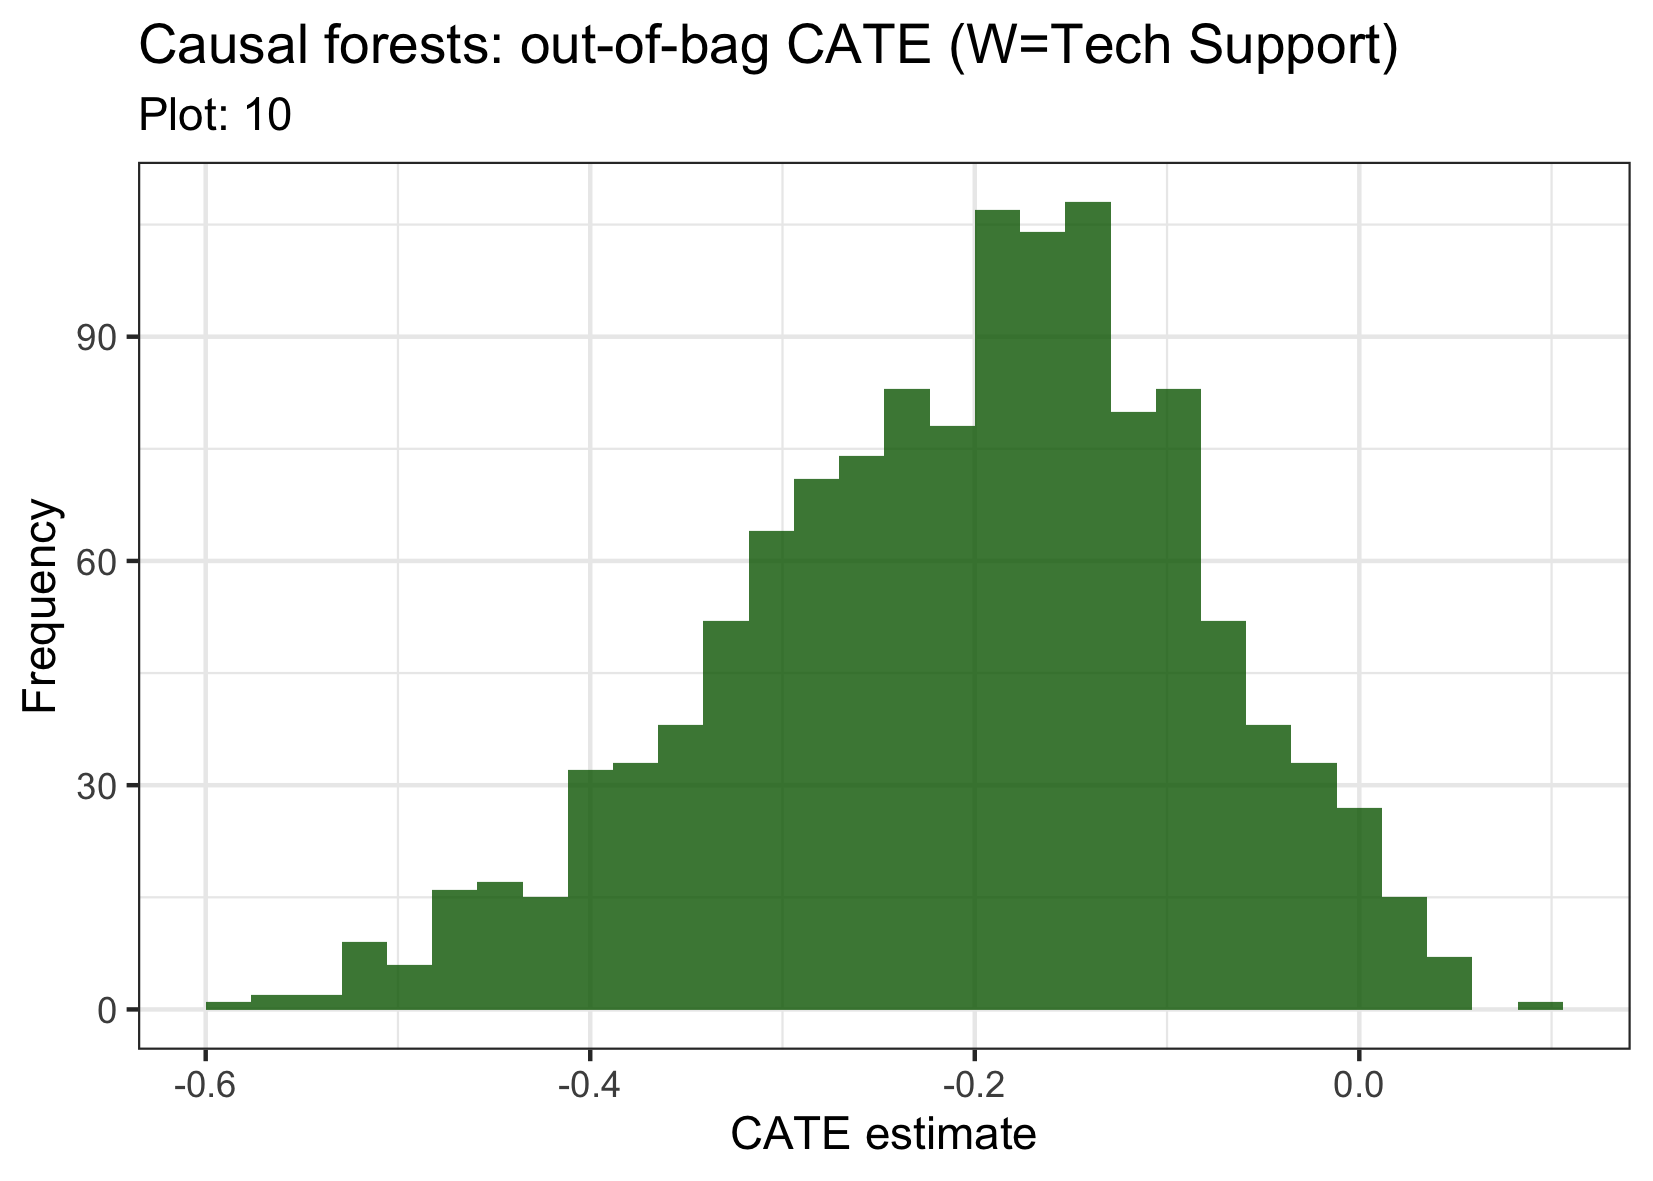
\includegraphics[scale=0.15]{chinchilab-template/chapters/appendices/ANALYSIS/CATE_10.png}
    \caption{Distribution of CATE (Model 10)}
    \label{fig:my_label}
\end{figure}

%%%%%%%%%%%%%%%%%%%%%%%%%%%%%%%%%%%%%%%%%%%%%%%%%%%%%%%%%%%%
\section{C.2.3.1 Matching Quality}
%%%%%%%%%%%%%%%%%%%%%%%%%%%%%%%%%%%%%%%%%%%%%%%%%%%%%%%%%%%%

\begin{table}[H]
\centering
\footnotesize
\caption{Balance Check for USDEUR Subset}
\begin{tabular}{lllll}
\\[-1.8ex]\hline 
\hline \\[-1.8ex] 
Variables & Std. Mean Diff. (Pre) & Std. Mean Diff. (Post) & eCDF Max (Pre) & eCDF Max (Post) \\
 \hline \\[-1.8ex] 
distance & 0.5507 & 0.2331 & 0.2566 & 0.0994 \\
MTG & -0.1206 & -0.0491 & 0.0306 & 0.0128 \\
SEC & -0.4233 & -0.1202 & 0.0164 & 0.0048 \\
SR & 0.1917 & -0.0142 & 0.0849 & 0.0064 \\
SRBN & 0.1307 & 0.1112 & 0.0311 & 0.0272 \\
SRP & 0.0971 & 0.0468 & 0.0259 & 0.0128 \\
SRSEC & -0.1956 & -0.0394 & 0.0309 & 0.0064 \\
SRSUB & -0.0322 & 0.0000 & 0.0013 & 0.0000 \\
SUB & -0.1733 & 0.0360 & 0.0150 & 0.0032 \\
UN & -0.3018 & -0.0788 & 0.0477 & 0.0128 \\
Time to Maturity (Days) & 0.1856 & 0.0916 & 0.1569 & 0.0593 \\
Guarantor & -0.1357 & -0.0360 & 0.0471 & 0.0128 \\
Euro & 0.1921 & 0.0519 & 0.0890 & 0.0240 \\
U.S. Dollar & -0.1921 & -0.0519 & 0.0890 & 0.0240 \\
A & 0.2108 & 0.0702 & 0.0884 & 0.0288 \\
AA & -0.0967 & -0.0693 & 0.0397 & 0.0288 \\
AAA & -0.3147 & -0.0621 & 0.1458 & 0.0288 \\
B & 0.0131 & 0.0567 & 0.0007 & 0.0032 \\
BB & 0.0040 & -0.0712 & 0.0005 & 0.0080 \\
BBB & 0.2281 & 0.0799 & 0.0959 & 0.03 \\
\hline \\[-1.8ex] 
\end{tabular}
\caption*{Before Matching: Brown Bonds: 4349, Green Bonds: 663 \\
After Matching: Brown Bonds: 624, Green Bonds 624.}
\end{table}


\newpage

%%%%%%%%%%%%%%%%%%%%%%%%%%%%%%%%%%%%%%%%%%%%%%%%%%%%%%%%%%%%
\section{C.2.3.1 Nuisance Parameter Check}
%%%%%%%%%%%%%%%%%%%%%%%%%%%%%%%%%%%%%%%%%%%%%%%%%%%%%%%%%%%%

\begin{figure}[H]
    \centering
    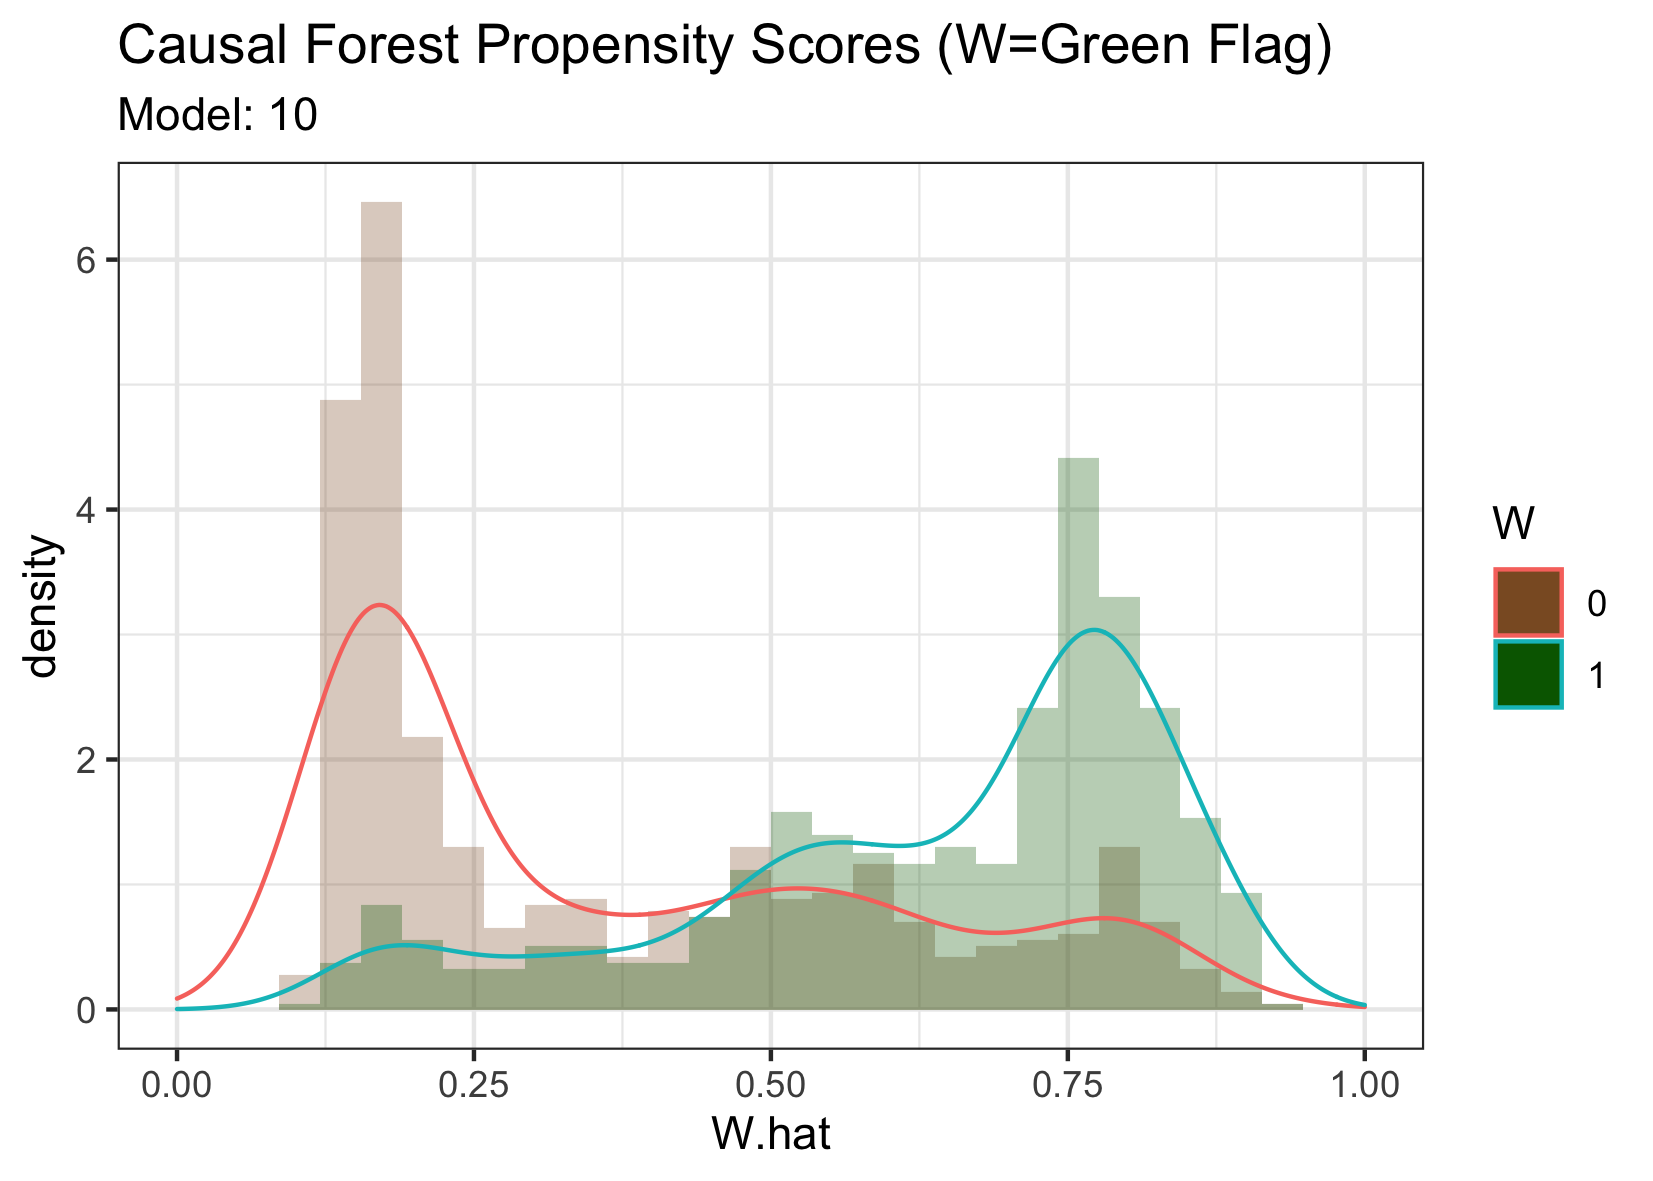
\includegraphics[scale=.15]{chinchilab-template/chapters/appendices/ANALYSIS/prop_10.png}
    \caption{Propensity Score Distribution for Model 10}
    \label{fig:my_label}
\end{figure}


\begin{table}[H]{
    \begin{subtable}{.5\textwidth}
    \centering
    \footnotesize
        {\begin{tabular}{@{\extracolsep{5pt}}lc} 
        \\[-1.8ex]\hline 
        \hline \\[-1.8ex] 
         & \multicolumn{1}{c}{\textit{Dependent variable: Green Flag}} \\ 
        \cline{2-2} 
        \\[-1.8ex] &   \\ 
        \hline \\[-1.8ex] 
         e.bar & 1.000$^{***}$ \\ 
          & (0.024) \\ 
          & \\ 
         e.residual & 1.075$^{***}$ \\ 
          & (0.041) \\ 
          & \\ 
        \hline \\[-1.8ex] 
        \hline 
        \hline \\[-1.8ex] 
        \textit{Note:}  & \multicolumn{1}{r}{$^{*}$p$<$0.1; $^{**}$p$<$0.05; $^{***}$p$<$0.01} \\ 
        \end{tabular} }
    \subcaption{Outcome Model}
    \end{subtable}
    \begin{subtable}{0.3\linewidth}
    \centering
    \footnotesize
        {\begin{tabular}{@{\extracolsep{5pt}}lc} 
        \\[-1.8ex]\hline 
        \hline \\[-1.8ex] 
         & \multicolumn{1}{c}{\textit{Dependent variable: Green Flag}} \\ 
        \cline{2-2} 
        \\[-1.8ex] &   \\ 
        \hline \\[-1.8ex] 
         m.bar & 0.999$^{***}$ \\ 
          & (0.015) \\ 
          & \\ 
         m.residual & 1.302$^{***}$ \\ 
          & (0.031) \\ 
          & \\ 
        \hline \\[-1.8ex] 
        \hline 
        \hline \\[-1.8ex] 
        \textit{Note:}  & \multicolumn{1}{r}{$^{*}$p$<$0.1; $^{**}$p$<$0.05; $^{***}$p$<$0.01} \\ 
        \end{tabular}}
    \subcaption{Propensity Model}
    \end{subtable}
\caption{Calibration Regressions (Model 10)}
\label{x}}
\end{table}


%%%%%%%%%%%%%%%%%%%%%%%%%%%%%%%%%%%%%%%%%%%%%%%%%%%%%%%%%%%%
\subsubsection{C.2.3.2 Heterogeneity Assessment}
%%%%%%%%%%%%%%%%%%%%%%%%%%%%%%%%%%%%%%%%%%%%%%%%%%%%%%%%%%%%

\begin{table}[h!]
\centering
\caption{Variable Importance (Model 10)}
\begin{tabular}{lr}
\\[-1.8ex]\hline 
\hline \\[-1.8ex] 
\rowcolor[HTML]{FFFFFF} 
{\color[HTML]{333333} \textbf{Covariate}} & {\color[HTML]{333333} \textbf{Value}} \\ \hline
\rowcolor[HTML]{FFFFFF} 
{\color[HTML]{333333} Issue Amount} & \cellcolor[HTML]{00441B}{\color[HTML]{FFFFFF} 0.29489032} \\
\rowcolor[HTML]{FFFFFF} 
{\color[HTML]{333333} Time to Maturity (Days)} & \cellcolor[HTML]{30984F}{\color[HTML]{FFFFFF} 0.21820993} \\
\rowcolor[HTML]{FFFFFF} 
{\color[HTML]{333333} 2022} & \cellcolor[HTML]{EFF9EC}{\color[HTML]{FFFFFF} 0.05453479} \\
\rowcolor[HTML]{FFFFFF} 
{\color[HTML]{333333} 2020} & \cellcolor[HTML]{F4FBF1}{\color[HTML]{333333} 0.04649319} \\
\rowcolor[HTML]{FFFFFF} 
{\color[HTML]{333333} Financials} & \cellcolor[HTML]{F7FCF5}{\color[HTML]{333333} 0.04166802} \\
\rowcolor[HTML]{FFFFFF} 
{\color[HTML]{333333} 2018} & \cellcolor[HTML]{F7FCF5}{\color[HTML]{333333} 0.04093371} \\ \hline
\end{tabular}
\end{table}

\begin{figure}[h!]
    \centering
    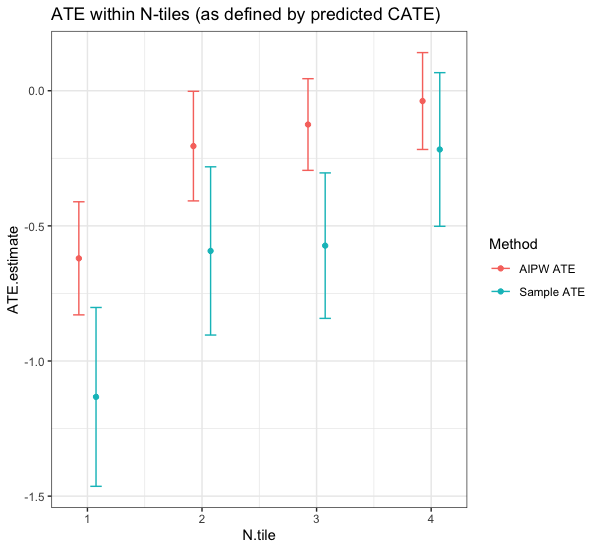
\includegraphics[scale=0.4]{chinchilab-template/chapters/appendices/ANALYSIS/ntile_cf23.png}
    \caption{Graph of ATE within Subgroups (Model 10)}
    \label{fig:my_label}
\end{figure}

\begin{figure}[H]
\centering
   \begin{subfigure}[b]{0.45\textwidth}
    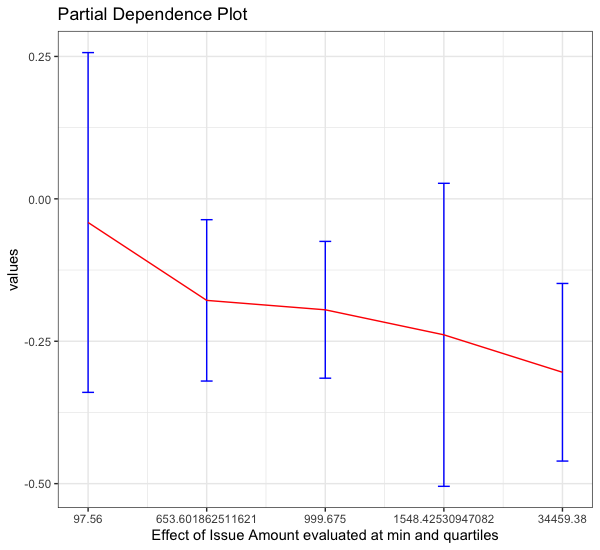
\includegraphics[width=0.8\textwidth]{chinchilab-template/chapters/appendices/ANALYSIS/PDP_cf23.png}
    \caption{Effect of Issue Amount}
   \label{fig:Ng1} 
\end{subfigure}
\begin{subfigure}[b]{0.45\textwidth}
    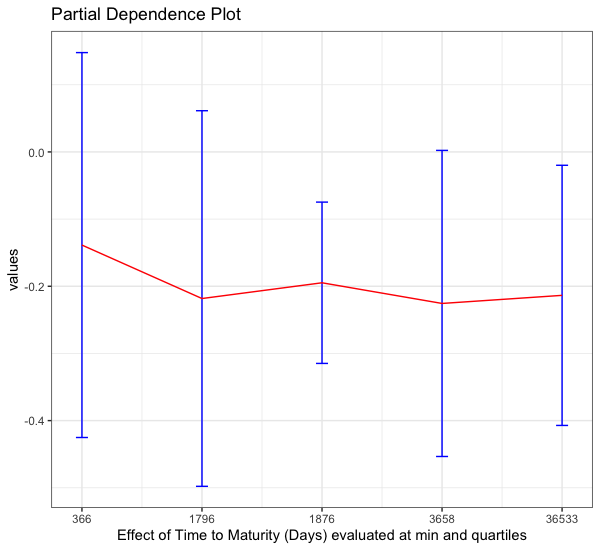
\includegraphics[width=0.8\textwidth]{chinchilab-template/chapters/appendices/ANALYSIS/PDP2_cf23.png}
    \caption{Effect of Time to Maturity (Days)}
   \label{fig:Ng2}
\end{subfigure}
\\
\begin{subfigure}[b]{0.45\textwidth}
    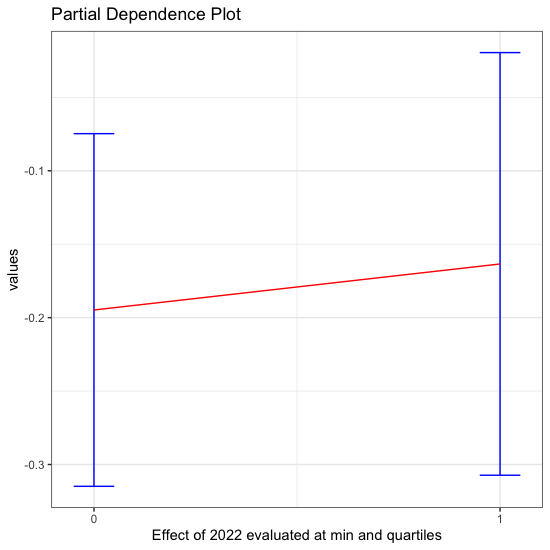
\includegraphics[width=0.8\textwidth]{chinchilab-template/chapters/appendices/ANALYSIS/PDP3_cf23.png}
    \caption{Effect of 2022}
   \label{fig:Ng2}
\end{subfigure}
\caption{Partial Dependency Plots (Model 10)}
\end{figure}


\begin{table}[H]
\caption{Heterogeneity across Covariates (Model 10)}
\label{Het}
\footnotesize
\begin{tabular}{lllll}
\\[-1.8ex]\hline 
\hline \\[-1.8ex] 
{\color[HTML]{333333} \textbf{Variable}} & {\color[HTML]{333333} \textbf{Mean ntile1}} & {\color[HTML]{333333} \textbf{Mean ntile2}} & {\color[HTML]{333333} \textbf{Mean ntile3}} & {\color[HTML]{333333} \textbf{Mean ntile4}} \\
\hline \\[-1.8ex] 
Time to   Maturity (Days) & \cellcolor[HTML]{63BE7B}3478.94 & \cellcolor[HTML]{95D3A6}3071.5 & \cellcolor[HTML]{C2E5CD}2698.03 & \cellcolor[HTML]{FCFCFF}2218.26 \\
Issue Amount & \cellcolor[HTML]{63BE7B}1982.47 & \cellcolor[HTML]{8ACE9D}1664.78 & \cellcolor[HTML]{D8EEE0}1026.88 & \cellcolor[HTML]{FCFCFF}732.29 \\
Guarantor & \cellcolor[HTML]{DEF0E5}0.18 & \cellcolor[HTML]{DEF0E5}0.18 & \cellcolor[HTML]{E3F2EA}0.15 & \cellcolor[HTML]{E8F4EE}0.12 \\
2013 & \cellcolor[HTML]{EFF7F4}0.08 & \cellcolor[HTML]{F7FAFB}0.03 & \cellcolor[HTML]{F7FAFB}0.03 & \cellcolor[HTML]{F7FAFB}0.03 \\
2014 & \cellcolor[HTML]{EDF6F2}0.09 & \cellcolor[HTML]{F6FAFA}0.04 & \cellcolor[HTML]{F7FAFB}0.03 & \cellcolor[HTML]{FBFCFE}0.01 \\
2015 & \cellcolor[HTML]{F4F9F8}0.05 & \cellcolor[HTML]{F4F9F8}0.05 & \cellcolor[HTML]{F4F9F8}0.05 & \cellcolor[HTML]{ECF6F1}0.1 \\
2016 & \cellcolor[HTML]{EDF6F2}0.09 & \cellcolor[HTML]{F2F8F7}0.06 & \cellcolor[HTML]{F2F8F7}0.06 & \cellcolor[HTML]{EFF7F4}0.08 \\
2017 & \cellcolor[HTML]{F6FAFA}0.04 & \cellcolor[HTML]{F2F8F7}0.06 & \cellcolor[HTML]{E8F4EE}0.12 & \cellcolor[HTML]{E5F3EB}0.14 \\
2018 & \cellcolor[HTML]{F6FAFA}0.04 & \cellcolor[HTML]{E8F4EE}0.12 & \cellcolor[HTML]{ECF6F1}0.1 & \cellcolor[HTML]{EAF5F0}0.11 \\
2019 & \cellcolor[HTML]{EFF7F4}0.08 & \cellcolor[HTML]{E5F3EB}0.14 & \cellcolor[HTML]{E3F2EA}0.15 & \cellcolor[HTML]{EDF6F2}0.09 \\
2020 & \cellcolor[HTML]{F4F9F8}0.05 & \cellcolor[HTML]{EFF7F4}0.08 & \cellcolor[HTML]{E5F3EB}0.14 & \cellcolor[HTML]{E5F3EB}0.14 \\
2021 & \cellcolor[HTML]{E3F2EA}0.15 & \cellcolor[HTML]{DEF0E5}0.18 & \cellcolor[HTML]{E3F2EA}0.15 & \cellcolor[HTML]{F2F8F7}0.06 \\
2022 & \cellcolor[HTML]{EFF7F4}0.08 & \cellcolor[HTML]{E8F4EE}0.12 & \cellcolor[HTML]{ECF6F1}0.1 & \cellcolor[HTML]{DDF0E4}0.19 \\
Annual Coupon & \cellcolor[HTML]{71C487}0.83 & \cellcolor[HTML]{8CCF9E}0.67 & \cellcolor[HTML]{8FD0A1}0.65 & \cellcolor[HTML]{8FD0A1}0.65 \\
Semi Annual   Coupon & \cellcolor[HTML]{E0F1E7}0.17 & \cellcolor[HTML]{C7E7D1}0.32 & \cellcolor[HTML]{C2E5CD}0.35 & \cellcolor[HTML]{C2E5CD}0.35 \\
Quarterly & \cellcolor[HTML]{FCFCFF}0 & \cellcolor[HTML]{FCFCFF}0 & \cellcolor[HTML]{FCFCFF}0 & \cellcolor[HTML]{FCFCFF}0 \\
Senior   Secured Mortgage & \cellcolor[HTML]{FBFCFE}0.01 & \cellcolor[HTML]{F2F8F7}0.06 & \cellcolor[HTML]{E8F4EE}0.12 & \cellcolor[HTML]{E5F3EB}0.14 \\
Senior Secured & \cellcolor[HTML]{F9FBFD}0.02 & \cellcolor[HTML]{F9FBFD}0.02 & \cellcolor[HTML]{F6FAFA}0.04 & \cellcolor[HTML]{F6FAFA}0.04 \\
Senior Unsecured & \cellcolor[HTML]{63BE7B}0.91 & \cellcolor[HTML]{7EC993}0.75 & \cellcolor[HTML]{94D2A6}0.62 & \cellcolor[HTML]{99D4AA}0.59 \\
Senior Non   Preferred & \cellcolor[HTML]{FBFCFE}0.01 & \cellcolor[HTML]{F4F9F8}0.05 & \cellcolor[HTML]{EFF7F4}0.08 & \cellcolor[HTML]{F2F8F7}0.06 \\
Senior Preferred & \cellcolor[HTML]{FBFCFE}0.01 & \cellcolor[HTML]{F2F8F7}0.06 & \cellcolor[HTML]{E8F4EE}0.12 & \cellcolor[HTML]{EAF5F0}0.11 \\
Senior   Subordinated Unsecured & \cellcolor[HTML]{FCFCFF}0 & \cellcolor[HTML]{FCFCFF}0 & \cellcolor[HTML]{FCFCFF}0 & \cellcolor[HTML]{FCFCFF}0 \\
Subordinated   Unsecured & \cellcolor[HTML]{FCFCFF}0 & \cellcolor[HTML]{FBFCFE}0.01 & \cellcolor[HTML]{FCFCFF}0 & \cellcolor[HTML]{FBFCFE}0.01 \\
Basic Materials & \cellcolor[HTML]{F6FAFA}0.04 & \cellcolor[HTML]{FCFCFF}0 & \cellcolor[HTML]{FBFCFE}0.01 & \cellcolor[HTML]{FBFCFE}0.01 \\
Consumer   Cyclicals & \cellcolor[HTML]{F9FBFD}0.02 & \cellcolor[HTML]{FCFCFF}0 & \cellcolor[HTML]{FCFCFF}0 & \cellcolor[HTML]{FCFCFF}0 \\
Consumer   Non Cyclicals & \cellcolor[HTML]{F9FBFD}0.02 & \cellcolor[HTML]{FBFCFE}0.01 & \cellcolor[HTML]{FCFCFF}0 & \cellcolor[HTML]{FCFCFF}0 \\
Energy & \cellcolor[HTML]{FBFCFE}0.01 & \cellcolor[HTML]{FCFCFF}0 & \cellcolor[HTML]{FCFCFF}0 & \cellcolor[HTML]{FCFCFF}0 \\
Financials & \cellcolor[HTML]{C5E6D0}0.33 & \cellcolor[HTML]{9BD5AB}0.58 & \cellcolor[HTML]{80CA94}0.74 & \cellcolor[HTML]{71C487}0.83 \\
Healthcare & \cellcolor[HTML]{FBFCFE}0.01 & \cellcolor[HTML]{FCFCFF}0 & \cellcolor[HTML]{FCFCFF}0 & \cellcolor[HTML]{FCFCFF}0 \\
Industrials & \cellcolor[HTML]{F6FAFA}0.04 & \cellcolor[HTML]{F9FBFD}0.02 & \cellcolor[HTML]{F7FAFB}0.03 & \cellcolor[HTML]{F7FAFB}0.03 \\
Institutions,   Associations \& Organizations & \cellcolor[HTML]{EDF6F2}0.09 & \cellcolor[HTML]{EDF6F2}0.09 & \cellcolor[HTML]{F6FAFA}0.04 & \cellcolor[HTML]{F7FAFB}0.03 \\
Real Estate & \cellcolor[HTML]{FBFCFE}0.01 & \cellcolor[HTML]{FCFCFF}0 & \cellcolor[HTML]{FCFCFF}0 & \cellcolor[HTML]{FBFCFE}0.01 \\
Technology & \cellcolor[HTML]{F9FBFD}0.02 & \cellcolor[HTML]{FBFCFE}0.01 & \cellcolor[HTML]{FCFCFF}0 & \cellcolor[HTML]{FCFCFF}0 \\
Utilities & \cellcolor[HTML]{EDF6F2}0.09 & \cellcolor[HTML]{F6FAFA}0.04 & \cellcolor[HTML]{F6FAFA}0.04 & \cellcolor[HTML]{F9FBFD}0.02 \\
AAA & \cellcolor[HTML]{C7E7D1}0.32 & \cellcolor[HTML]{BBE2C7}0.39 & \cellcolor[HTML]{C3E5CE}0.34 & \cellcolor[HTML]{CFEAD8}0.27 \\
AA & \cellcolor[HTML]{DEF0E5}0.18 & \cellcolor[HTML]{DEF0E5}0.18 & \cellcolor[HTML]{D2EBDB}0.25 & \cellcolor[HTML]{C3E5CE}0.34 \\
A & \cellcolor[HTML]{DEF0E5}0.18 & \cellcolor[HTML]{DEF0E5}0.18 & \cellcolor[HTML]{D8EEE0}0.22 & \cellcolor[HTML]{D8EEE0}0.22 \\
BBB & \cellcolor[HTML]{CCE9D5}0.29 & \cellcolor[HTML]{D4ECDD}0.24 & \cellcolor[HTML]{E2F2E8}0.16 & \cellcolor[HTML]{E0F1E7}0.17 \\
BB & \cellcolor[HTML]{F7FAFB}0.03 & \cellcolor[HTML]{F9FBFD}0.02 & \cellcolor[HTML]{F9FBFD}0.02 & \cellcolor[HTML]{FBFCFE}0.01 \\
EUR & \cellcolor[HTML]{74C58A}0.81 & \cellcolor[HTML]{8CCF9E}0.67 & \cellcolor[HTML]{94D2A6}0.62 & \cellcolor[HTML]{98D4A8}0.6 \\
\hline \\[-1.8ex] 
\end{tabular}
\end{table}